\documentclass[journal]{IEEEtran}

\usepackage[utf8]{inputenc}
\usepackage[T1]{fontenc}
\usepackage{amsmath,amssymb,amsfonts}
\usepackage{graphicx}
\usepackage{booktabs}
\usepackage{array}
\usepackage{cite}
\usepackage{url}
\usepackage{balance}

\graphicspath{{results/}}

\newtheorem{theorem}{Theorem}
\newtheorem{corollary}{Corollary}
\newtheorem{proposition}{Proposition}

\begin{document}

\title{A Behavior-Coordinate Realization Interface for Predictive Saturation Management}

\author{Yongyan~Cao %
\thanks{Y.~Cao is with Voryx Robotics LLC, San Jose, CA 95136, USA (e-mail: yongyancao@gmail.com).}%
}

\markboth{Preprint}%
{Cao: A Behavior-Coordinate Realization Interface for Predictive Saturation Management}

\maketitle

\begin{abstract}
When a robot controller requests behavior its actuators cannot realize, torque clipping keeps the
hardware command legal but silently changes the behavior executed: the robot is no longer running
the PD, impedance, or learned law that was designed or trained, and nothing in the loop announces
it. This matters directly in physical interaction, where the requested acceleration sets apparent
compliance and disturbance response. We present a behavior-coordinate realization interface that
detects and corrects this condition before clipping is reached. Heterogeneous nominal controllers
expose a common task-acceleration request at servo rate; a slower manager reconstructs the
executing robot's configuration-dependent torque-feasible set, predicts loss of realizability over
a short horizon, and returns a minimum-cost correction in the same behavior coordinates, with a
fast projection retained as a last-resort actuator guard. The interface is designed to be
auditable in deployment: three measurable conditions --- torque-prediction accuracy, actuator
margin, and behavior-successor mismatch --- decide online whether the acceleration-to-torque
interface can currently be trusted, and a one-step result establishes that the behavior
certificate is preserved whenever they hold. A corollary gives the additional torque-drift and
averaged-request conditions required by the two-rate implementation.
A 111-run deterministic study evaluates the interface across five nominal-controller forms, three
realization maps, eight stress scenarios, and a matched horizon trajectory-reference governor.
Full-horizon enforcement removes a 3.587~Nm predicted future torque violation and 31.180~mm of
workspace excess that first-step-only enforcement leaves behind. Under held-out plant
perturbations the audit reports positive margins with maximum $\ell_\infty$ successor defects
below 0.0069~m/s against a 0.03~m/s budget across all three realization maps. Against the matched
governor the proposed vector correction attains lower correction RMSE in three of the four
non-failure cases. The study also reports the conditions under which the interface fails:
abrupt disturbance and severe model mismatch violate the audit premises for both predictive
architectures, leaving only the reactive fallback. The benchmark is reduced-order and synthetic;
scope and the resulting limits on generality are stated in Section~\ref{sec:discussion}.
\end{abstract}

\begin{IEEEkeywords}
Physical interaction, actuator saturation, behavior-coordinate interface, predictive constraint management, control refinement.
\end{IEEEkeywords}

\section{Introduction}
\label{sec:intro}

\IEEEPARstart{A}{} controller computes a torque request $\tau^0$ and the hardware applies
\[
\tau^{\mathrm{app}}
=
\operatorname{clip}\left(\tau^0,\ \tau_{\min},\ \tau_{\max}\right),
\]
that is, each joint's torque is pushed back to its nearest limit whenever the request exceeds it. The clip protects the actuator. It does not protect the behavior. Once the clip is active, the acceleration the robot produces is not the acceleration the controller asked for, so the robot is no longer running the PD, impedance, or learned law that was designed or trained. Nothing in the loop announces this. The controller keeps issuing requests, the actuators keep saturating, and the realized closed-loop dynamics silently drift away from the intended ones. In physical interaction this matters directly, because the requested acceleration is what sets apparent compliance and disturbance response.

Different controllers reach this state through different routes. A fixed-gain PD law gets there through a large tracking error. An impedance law $M_d\ddot e=-K_de-D_d\dot e+F_h$ gets there through contact force, even when tracking error is small. A $\tanh$-squashed learned policy bounds its requested \emph{acceleration}, but the torque that acceleration implies depends on the configuration, so a bound on the request is not a bound on the torque. An upstream language- or diffusion-conditioned module may propose a motion primitive with no representation of the executing robot's actuator limits at all. The route differs; the failure is the same.

Keep the nominal controller unchanged, but require it to expose a task-acceleration request. Add a much slower layer that predicts whether each robot can realize that request and outputs a correction in the same behavior coordinates.

\begin{quote}
\emph{The nominal controller runs unchanged at its own high servo rate. A much slower manager rolls its behavior request forward over a short horizon, reconstructs the executing robot's torque-feasible acceleration set, and, when its QP is feasible, applies a minimum-cost correction to the requested acceleration before hard clipping is required.}
\end{quote}

The manager does not choose the task and does not replace the controller. Because its job is to predict and correct rather than react, it also does not need to run at servo rate; how slow it can run in general depends on the operating region and model (a concrete rate pair is instantiated in Section~\ref{sec:experiments}). Its only job is to keep the request physically producible while staying as close as possible to what the controller asked for. A final high-rate projection stays in place for disturbances that arrive between manager updates; prediction and last-resort protection are separate responsibilities, and Section~\ref{sec:experiments} shows they can be needed at different moments.

A one-step check answers ``is the command legal right now?'' That is not the same question as ``does this planned sequence remain legal?'' Position and velocity carry forward, so a future constraint can require changing acceleration before the limiting step arrives. This distinction is standard in predictive constraint management \cite{r3,r5,r16,r17,r18}. Fig.~\ref{fig:horizon} isolates its role inside the proposed interface: constraining every predicted move eliminates the planned torque excess in the horizon-ramp case, while constraining only the first move leaves a 3.587~Nm future violation and 31.180~mm of workspace excess (Section~\ref{sec:anticipatory}).

Feedback linearization to a double-integrator-like behavior model is classical \cite{r1,r2}. Reference governors, generalized action governors, predictive safety filters, anti-windup control, model-predictive constraint handling, and task-space capacity polytopes are established \cite{r3,r4,r5,r6,r7,r16,r17,r18,r19,r20}; the double integrator, the QP, and the ray-to-polytope authority calculation are used here as implementation ingredients. The contribution is their arrangement into an auditable interface, described next.

The question we do ask is this:

\begin{quote}
Can a common behavior-acceleration request be supervised without hiding robot-specific actuator geometry, and can the boundary between behavior preservation and physical realization be stated as quantities that an implementation can audit?
\end{quote}

The proposed answer is an interface decomposition, not a new class of constrained controller. Behavior dynamics provide the shared request and certificate coordinates; the torque map, feasible set, and uncertainty bounds remain robot-specific. Section~\ref{sec:certificate} specializes existing refinement logic \cite{r8,r9,r19} to three quantities that expose when this particular acceleration-to-torque interface can be trusted.

\textbf{Contributions.}
\begin{enumerate}
\item A behavior-coordinate realization interface in which heterogeneous nominal controllers expose the same task-acceleration request while every executing robot retains its own configuration-dependent acceleration-to-torque map and feasible set.
\item A two-rate implementation that corrects the behavior request predictively, recomputes the robot-specific realization map on the fast path, and reports both scalar torque headroom and directional acceleration authority; the components are assembled to preserve the interface across heterogeneous controllers and robots.
\item An actuator-realization specialization of one-step certificate refinement, separating torque-prediction accuracy (T1), actuator margin (T2), and behavior-successor mismatch (T3), together with a minimal velocity-certified action set enforced in the QP. A separate corollary states the additional torque-drift and averaged-request conditions needed by the two-rate implementation. These are conditions an implementation can evaluate online.
\item A reproducible 111-run reduced-order study, including a matched horizon trajectory-reference-governor comparison, deterministic held-out plant perturbations, repeated anchor cases across matrices, five controller interfaces, three realization maps, eight stress scenarios, the T1--T3 audit, and explicit negative cases (parameters and complete artifacts in the supplementary archive).
\end{enumerate}

The experiments establish internal operation and failure detection for this interface. The implemented comparison is an ERG-style 
finite-horizon trajectory-reference governor matched in model and computation budget, not an exact reproduction of the 
Lyapunov/dynamic-safety-margin construction in \cite{r17}. The experiments therefore do not establish that other 
reference/action governors or predictive safety filters cannot implement the same behavior coordinates.

\textbf{Notation.} Everything in the paper uses the following symbols. All vector inequalities are componentwise (joint by joint).

\begin{table}[t]
\caption{Notation}
\label{tab:notation}
\centering
\footnotesize
\setlength{\tabcolsep}{3pt}
\begin{tabular}{@{}p{1.65cm}p{5.05cm}p{1.0cm}@{}}
\toprule
Symbol & Meaning in words & Units \\
\midrule
$\tau^0$ & torque the nominal controller asks for & Nm \\
$\tau^{\mathrm{pre}}$ & torque that would be sent \emph{before} any clipping & Nm \\
$\tau^{\mathrm{app}}$ & torque actually applied, after clipping & Nm \\
$\hat\tau$ & the manager's \emph{prediction} of $\tau^{\mathrm{pre}}$ & Nm \\
$\tau_{\min},\tau_{\max}$ & actuator limits & Nm \\
$\tau_{\mathrm{base}}$ & torque already spoken for: gravity, Coriolis, orientation, null-space & Nm \\
$F_h$ & measured interaction force & N \\
$G_F(x)$ & converts $F_h$ into task-acceleration units; general form $\Lambda^{-1}(x)$, this benchmark uses $\tfrac1m I$ & 1/kg \\
$a$ & requested task acceleration (the decision variable) & m/s$^2$ \\
$a^{0}$ & acceleration the nominal controller asks for & m/s$^2$ \\
$\Delta a=a-a^{0}$ & the correction the manager applies & m/s$^2$ \\
$p,v$ & task position and velocity, propagated directly & m, m/s \\
$z=[p;v]$ & task state & --- \\
$e_c=p-p_r(t)$ & a controller's own tracking error against its reference $p_r(t)$; internal to the controller, not part of $z$ & m \\
$\mathcal X$ & running workspace-and-speed box on $z$ & --- \\
$H(x)$ & maps a requested acceleration to the torque it costs & Nm\,s$^2$\!/m \\
$\mathcal A(x)$ & accelerations that are interface-realizable --- legal through $H(x)$ and $\tau_{\mathrm{base}}(x)$ --- at this configuration & m/s$^2$ \\
$\mathcal A^{\mathrm{tight}}(x)$ & same set, shrunk by the uncertainty margin & m/s$^2$ \\
$\bar\delta_\tau$ & how far the real torque can differ from the prediction & Nm \\
$\alpha^{+}$ & remaining acceleration authority in a given direction & m/s$^2$ \\
$\mathcal S_v=\{y:\|y\|_\infty\le v_{\max}\}$ & the certified velocity region & --- \\
$\epsilon_v$ & certificate margin: the one-step velocity error the certificate tolerates & m/s \\
$\mathcal K_v(y)$ & the certified action set: requests from $y$ that stay inside $\mathcal S_v$ after up to $\epsilon_v$ of error & m/s$^2$ \\
\bottomrule
\end{tabular}
\end{table}

Two set operations appear in Section~\ref{sec:certificate} only, and both have a plain reading: $\mathcal X\oplus\mathcal Y$ means ``any point of $\mathcal X$ plus any point of $\mathcal Y$'' (worst case over both), and $\mathcal X\subseteq\mathcal Y$ means ``$\mathcal X$ fits inside $\mathcal Y$.''

\section{How the Method Works}
\label{sec:howitworks}

This section walks through the loop once, before any of it is formalized.

\textbf{Fast loop, at the controller's own high servo rate $T_f$, regardless of which controller is in use.} Evaluate the nominal controller to get its requested acceleration $a^0$, converted to torque $\tau^0$ through the realization map (Section~\ref{sec:realizable}). Add the latest correction published by the manager, converted to torque at the \emph{current} configuration:
\[
\tau^{\mathrm{pre}}=\underbrace{\tau^0}_{\text{controller}}+\underbrace{H(x)\,\Delta a}_{\text{manager's correction}},
\]
then apply the final high-rate projection, the last-resort guard,
\[
\tau^{\mathrm{app}}=\operatorname{clip}\left(\tau^{\mathrm{pre}},\ \tau_{\min},\ \tau_{\max}\right),
\]
which is what is sent to the robot.

\textbf{Slow loop, every manager period $\Delta t$, much longer than $T_f$.} The manager publishes a correction in \emph{acceleration}, not a cached torque; $H(x)$ is recomputed on every fast-loop tick, so configuration drift between manager updates does not turn a stale plan into an artificial disturbance. Each update:
\begin{enumerate}
\item Roll the nominal controller forward $N=12$ steps to get the requested accelerations $a^0_0,\dots,a^0_{N-1}$ and the predicted states.
\item At each predicted state, build the set of accelerations the robot can actually realize, shrunk by the uncertainty margin.
\item Solve one small QP for the acceleration sequence closest to the nominal request that stays inside those sets, inside the workspace box, and inside the velocity-certificate set of Section~\ref{sec:certificate}.
\item Publish the first-step correction $\Delta a$; log the margin and directional authority.
\end{enumerate}

If the nominal rollout is already feasible everywhere, the QP returns the nominal request and the correction is zero --- the manager is inactive during ordinary operation.

\textbf{Where the anticipation lives.} There is no separate ``saturation detector.'' Along the nominal rollout the predicted torque is $\hat\tau=\tau_{\mathrm{base}}+H(a^{0}-G_F\hat F_h)$; when that torque enters the tightened boundary layer at any step of the horizon, the corresponding constraint becomes active and the QP is forced to move. The tightening is what makes the constraint bite \emph{early}; the forward propagation of position and velocity is what turns a future activation into a present correction.

\section{Related Work and Positioning}
\label{sec:related}

Impedance control specifies a desired motion--force relation \cite{r1}, and operational-space control maps task accelerations or wrenches to joint torque \cite{r2}. Both rely on adequate actuator authority. Anti-windup methods treat saturation-induced degradation inside a particular closed loop \cite{r6,r7}, while model-reference adaptive impedance control seeks to reproduce a target impedance despite uncertain dynamics \cite{r11}. Interaction-control MPC methods instead adapt impedance parameters or trajectories using learned interaction dynamics, Gaussian processes, or environment estimates \cite{r12,r13,r14,r15}. The present work does not replace these controllers: it requires an upstream controller to expose a task-acceleration request and supervises whether a robot can realize it.

Reference and command governors are established add-on mechanisms that modify a reference to keep a pre-stabilized system 
within constraints \cite{r3}. Ambrosino \emph{et al.} directly addressed robotic actuator saturation with a trajectory-based explicit reference governor, retaining an internal PD controller and validating position, velocity, and saturation handling on a seven-degree-of-freedom KUKA arm \cite{r17}. Generalized action governors move the supervisor after the controller, modify an action rather than a reference, and provide all-time constraint results through safe and returnable sets under bounded uncertainty \cite{r18}. Predictive safety filters similarly accept a nominal action, use a predictive model and uncertainty description, and minimally replace unsafe actions; their terminal safety policy supports a recursive guarantee absent here \cite{r5,r16}. 
Consequently, retaining a controller, predicting constraints, and minimizing action modification are prior art. 
Our design choice is the \emph{action representation}: heterogeneous controllers expose task acceleration, 
while a separate realization object maps it into configuration-dependent robot torque and exposes T1--T3 audit quantities.

Robot capability and acceleration polytopes already map joint torque boxes into task-space force or acceleration sets, and ray-to-boundary calculations already quantify directional capacity \cite{r20}. We use those ideas to construct $\mathcal A(x)$ and $\alpha^+$, not as new polytope theory, but as the robot-specific half of the behavior--realization interface.

The certificate argument likewise builds on approximate simulation, refinement, and contract-based design \cite{r8,r9,r10}. Recent transferred-control-barrier-function work uses simulation functions and explicit margins to transfer a certificate from a double integrator to full nonlinear quadrotor dynamics and enforce it with a QP filter \cite{r19}. That framework is more general and provides a substantive continuous-time transfer construction. Section~\ref{sec:certificate} instead gives a deliberately elementary discrete one-step specialization for actuator realization: T1 and T2 isolate whether a predicted behavior request survives the torque interface without clipping, and T3 isolates whether its physical successor stays within the behavior certificate's error budget.

Contact-oriented governors further show the breadth of modular constraint-management architectures. The compliant ERG of 
Gautam \emph{et al.} inserts a reference manager between planner and controller and uses an energy certificate for 
contact-friendly manipulation\cite{r21}. It differs in supervised variable and certificate, but reinforces why the present claim must be about a specific interface and audit decomposition rather than the existence of an add-on safety layer.

\begin{table*}[t]
\caption{Positioning Against the Closest Method Families}
\label{tab:positioning}
\centering
\footnotesize
\setlength{\tabcolsep}{4pt}
\begin{tabular}{@{}p{3.0cm}p{2.6cm}p{4.6cm}p{5.6cm}@{}}
\toprule
Approach & Quantity supervised & Main guarantee or evidence & Distinction from this work \\
\midrule
Saturation-aware trajectory ERG \cite{r17} & Joint reference & Predicted joint/velocity constraints and KUKA validation & Uses a PD-specific reference channel; no common behavior-acceleration/realization audit \\
Predictive safety filter \cite{r16} & Plant input/action & Uncertainty-aware predictive filtering with terminal safety policy & More general and recursively grounded; does not isolate the acceleration-to-torque T1--T3 interface \\
Generalized action governor \cite{r18} & Post-controller action & State/input constraints with safe-returnable-set guarantees & General action supervision; no robot task-acceleration realization object \\
Task-space capacity polytope \cite{r20} & Capability set, not a supervisor & Real-time force/velocity/acceleration capacity computation & Supplies geometry used here, but not the two-rate correction or interface contract \\
Transferred CBF \cite{r19} & Concrete-system safety-filter input & Simulation-function-based certificate transfer to nonlinear dynamics & General continuous-time transfer theory; not specialized to clipping and torque realizability \\
Compliant ERG \cite{r21} & Motion reference & Contact-energy certificate & Reference and energy interface rather than behavior acceleration and T1--T3 \\
This work & Task-acceleration request & Finite-horizon QP plus sampled one-step realization audit & Explicit behavior request/robot realization split; no recursive or hardware guarantee \\
\bottomrule
\end{tabular}
\\[2pt]
\raggedright\footnotesize Table I. Positioning against the closest method families. The comparison is architectural and theorem-level. Section~\ref{sec:experiments} additionally implements an ERG-style horizon trajectory-reference governor matched to this benchmark; it is not an exact reproduction of \cite{r17}.
\end{table*}

\section{What ``Realizable'' Means for a Given Robot}
\label{sec:realizable}

For a torque-controlled robot,
\[
M(q)\ddot q+h(q,\dot q)=\tau+J(q)^\top F_h,
\]
with $M(q)\succ0$, $h$ the modeled gravity/Coriolis/friction terms, and $F_h$ the measured interaction force (a two-dimensional vector in this benchmark, not a full wrench). Actuator limits are the box $\tau_{\min}\le\tau\le\tau_{\max}$.

The architecture asks only three things of the nominal controller: its \textbf{current requested task acceleration} $a^0$; an optional \textbf{preview}, i.e.\ the ability to be evaluated along a predicted trajectory; and a \textbf{bound on how wrong that preview can be}. An analytic PD or impedance law can be evaluated along predicted states directly. A learned policy can be queried on predicted observations. If no validated preview exists, zero-order hold or a learned predictor may be used, but the resulting error must be included in the bound. A black-box controller with neither query access nor a bounded preview error lies outside the certificate. The induced torque $\tau^0$ is obtained from $a^0$ through the realization map below.

With task state $z=[p;v]$ --- absolute task position and velocity, propagated directly rather than relative to a possibly time-varying reference --- the requested behavior over a local operating region is
\[
\ddot p=a+d_{\mathrm{res}},
\]
\emph{in words:} the acceleration the task actually realizes equals the requested acceleration plus a residual disturbance $d_{\mathrm{res}}$. Once the interaction-force compensation of \eqref{eq:iv0} below is introduced, $d_{\mathrm{res}}$ excludes $F_h$'s own (compensated) contribution and carries only what that compensation misses --- residual force-model error, cross-coupling, discretization --- checked explicitly as a one-step model error in Section~\ref{sec:certificate}. A reference-tracking controller may separately form its own tracking error $e_c=p-p_r(t)$ against a reference $p_r(t)$ to compute its request; this controller-internal error is not itself part of $z$.

Over one manager period this integrates to the constant-acceleration update
\[
p^{+}=p+\Delta t\,v+\tfrac12(\Delta t)^2(a+d_{\mathrm{res}}),
\qquad
v^{+}=v+\Delta t\,(a+d_{\mathrm{res}}),
\]
which is the standard $z^{+}=Az+B(a+d_{\mathrm{res}})$ double integrator. It is a shared interface, not a claimed novelty.

Realizing a requested acceleration $a$ costs torque. For the full-rigid-body model, let $N_\tau(q)\tau_{\mathrm{sec}}$ denote a dynamically consistent secondary torque satisfying $JM^{-1}N_\tau=0$. The bias and secondary contribution required by the operational-space realization is then
\begin{align}
\tau_{\mathrm{base}}(x)
&=J^\top\Lambda\bigl(JM^{-1}h-\dot J\dot q\bigr)
+N_\tau\tau_{\mathrm{sec}}, \nonumber\\
H(x)&=J(q)^\top\Lambda(q),
\quad
\Lambda=\left(JM^{-1}J^\top\right)^{-1}, \nonumber\\
G_F(x)&=\Lambda^{-1}(x).
\label{eq:iv0}
\end{align}
The commanded torque is
\begin{equation}
\tau=\tau_{\mathrm{base}}(x)+H(x)\,\bigl(a-G_F(x)F_h\bigr).
\label{eq:iv0a}
\end{equation}

Substitution into the robot dynamics gives $\ddot p=a$: the $JM^{-1}h$ and $\dot J\dot q$ terms cancel, the dynamically consistent secondary torque does not enter task acceleration, and $HG_FF_h=J^\top F_h$ cancels the modeled interaction-force term. Thus $a$ is the desired \emph{total} task acceleration, not a residual defined against a separate disturbance term. This remains conditional on the stated bias expression and dynamic consistency. Any omitted friction, imperfect bias term, non-decoupled secondary torque, or force-model error belongs in $d_{\mathrm{res}}$, $\bar\delta_\tau$, or the one-step mismatch bound rather than being silently absorbed by the identity. The reduced-order benchmark of Section~\ref{sec:experiments} does not claim this full derivation: it instantiates $\tau_{\mathrm{base}}$ and $H$ directly and uses the scalar approximation $G_F=\tfrac1m I$ (effective task-space mass $m$, Appendix~\ref{app:params}), exact only when $\Lambda\approx mI$.

We assume $J(q)$ has full row rank throughout the verified operating region and that $JM^{-1}J^\top$ is uniformly nonsingular there, $\lambda_{\min}(JM^{-1}J^\top)\ge\underline\lambda>0$; configurations violating this condition lie outside the certificate. A damped operational-space inverse may be used in implementation near such configurations, but its acceleration-realization defect must then be folded into $\bar\delta_\tau$ (torque domain) or the one-step model-error bound (velocity domain) rather than assumed away.

\emph{In words:} $H(x)$ is the price, in joint torque, of one unit of net task acceleration at this configuration, after the force compensation of \eqref{eq:iv0}. A request is realizable only if that price fits in the remaining budget:
\begin{equation}
\tau_{\min}\ \le\ \tau_{\mathrm{base}}(x)+H(x)\,(a-G_F(x)F_h)\ \le\ \tau_{\max}.
\label{eq:iv1}
\end{equation}

Call the set of $a$ satisfying \eqref{eq:iv1} the \textbf{feasible request set} $\mathcal A(x)$. This is the object that cannot be made robot-independent: it moves with the configuration through both $H(x)$ and $\tau_{\mathrm{base}}(x)$, and removing that dependence would remove exactly the geometry that causes saturation.

\textbf{Interface consistency.} The nominal interface supplies a requested task acceleration $a^0$, either directly --- as every controller evaluated in Section~\ref{sec:experiments} does --- or, for an opaque torque-only controller, through a robot-specific conversion satisfying the residual bound below. The induced nominal torque is
\[
\tau^0=\tau_{\mathrm{base}}(x)+H(x)\!\left(a^0-G_F(x)F_h\right)+r_\tau(x),
\]
\[
|r_\tau(x)|\le\bar r_\tau,
\]
where $r_\tau$ is an interface-consistency residual, bounded by the tightening margin $\bar\delta_\tau$ below; the five interfaces evaluated in Section~\ref{sec:experiments} are constructed so $r_\tau\equiv0$.

Condition~\eqref{eq:iv1} is a set of parallel slabs in $a$, one pair per joint, so $\mathcal A(x)$ is already a polytope in acceleration space.

Two practical consequences follow, and only these are used later.
\begin{itemize}
\item \textbf{It is not a ball.} Authority is direction-dependent. The robot can have plenty of torque left overall and still be nearly unable to accelerate along one particular direction.
\item \textbf{It is cheap to probe.} Directional authority is evaluated directly from the half-space representation of $\mathcal A^{\mathrm{tight}}(x)$, as defined in Section~\ref{sec:reports}; no vertex enumeration is required.
\end{itemize}

The manager predicts $\hat\tau$; the torque that would actually be sent, $\tau^{\mathrm{pre}}$, differs from it. Suppose that difference is bounded joint by joint:
\begin{equation}
\left|\tau^{\mathrm{pre}}-\hat\tau\right|\ \le\ \bar\delta_\tau.
\label{eq:iv2}
\end{equation}

Then it is not enough for the \emph{prediction} to sit inside the box; the prediction plus its error must. So the manager enforces the \textbf{tightened} condition
\begin{equation}
\tau_{\min}+\bar\delta_\tau\ \le\ \hat\tau\ \le\ \tau_{\max}-\bar\delta_\tau,
\label{eq:iv3}
\end{equation}
and we write $\mathcal A^{\mathrm{tight}}(x)$ for the accelerations satisfying it. Equation~\eqref{eq:iv3} is the whole tightening mechanism: a boundary layer of width $\bar\delta_\tau$ inside each actuator limit. It is what makes the constraint act \emph{before} the physical limit rather than at it, and Section~\ref{sec:ablation} shows what happens when it is removed.

The bound $\bar\delta_\tau$ must cover state-estimation error, interpolation between manager updates, secondary torque, torque-rate limiting (if present --- this implementation has none), and any other implementation effect that can move the pre-clip torque. The implementation uses two concrete instantiations of it: a conservative, action-independent $\bar\delta_\tau^{\mathrm{QP}}$, evaluated at the acceleration limit rather than the not-yet-chosen request, inside the QP's own tightening; and a smaller, action-dependent $\bar\delta_\tau(a,F_h)$, evaluated at the request actually solved for, used in the (T1) audit of Section~\ref{sec:experiments}. Since the QP's bound is evaluated at a worst-case acceleration, $\bar\delta_\tau^{\mathrm{QP}}\ge\bar\delta_\tau(a,F_h)$ over the acceleration box.

\textbf{Problem statement.} Given a nominal controller supplying $a^{0}$, find a correction $\Delta a$ such that:
\begin{enumerate}
\item $a=a^{0}+\Delta a$ stays close to the nominal request;
\item the realized torque stays inside the actuator box over the horizon, allowing for uncertainty;
\item the predicted state satisfies running workspace and speed constraints; and
\item the result can be tested against sufficient conditions for transferring an independently established behavior certificate.
\end{enumerate}

\section{The Predictive Correction and What the Manager Reports}
\label{sec:correction}

\subsection{The predictive correction}
\label{sec:predictivecorrection}

The nominal controller and the map $H(x)$ are evaluated, and the final torque-box projection applied, every fast-loop period $T_f$; the manager --- including the rate constraint on successive planned steps introduced below, which is evaluated only when the QP is solved --- runs every manager period $\Delta t$, much longer than $T_f$. Within one manager update we write $a_i$ for the request at horizon step $i=0,\dots,N-1$ and $a^0_i$ for what the nominal controller would ask there; the manager-update index is suppressed since everything below lives inside a single update. At $i=0$, $a_{-1}$ denotes the manager's own solved $a_0$ from the \emph{start} of the previous update, not that update's uncorrected nominal, so the rate constraint and smoothing term below bound change relative to the manager's own last decision.

The decision variable is the \emph{complete} request $a_i$, not the correction --- the constraints are physical conditions on the actual request, and the correction is read off afterwards. Subject to, for each $i$: a prediction row, a realizable-request row, a velocity-certificate row, a workspace row, and a request-rate row:
\small
\begin{align}
\min_{a_0,\dots,a_{N-1}}\quad
&\sum_{i=0}^{N-1}
\Big(
\underbrace{\|a_i-a^0_i\|^2_{W}}_{\text{stay close to the controller}}
+\underbrace{\|a_i-a_{i-1}\|^2_{W_\Delta}}_{\text{stay smooth}}
\Big)\nonumber\\[2pt]
& p_{i+1}=p_i+\Delta t\,v_i+\tfrac12(\Delta t)^2a_i,
\quad v_{i+1}=v_i+\Delta t\,a_i, \nonumber\\
& \tau_{\min}+\bar\delta_{\tau,i}^{\mathrm{QP}}\le\tau_{\mathrm{base}}(\hat x_i)+H(\hat x_i)\,(a_i-G_F(\hat x_i)\hat F_{h,i}) \nonumber\\
&\hspace{4.7em}\le\tau_{\max}-\bar\delta_{\tau,i}^{\mathrm{QP}}, \nonumber\\
& |v_i+\Delta t\,a_i|\le v_{\max}-\epsilon_v,
\quad z_{i+1}\in\mathcal X, \nonumber\\
& \|a_i\|_\infty\le a_{\max},
\quad
\|a_i-a_{i-1}\|_\infty\le\dot a_{\max}\Delta t.
\label{eq:qp}
\end{align}
\normalsize

Every constraint is linear in $a_i$ and the cost is convex quadratic, so this is a small dense QP. Here $\hat x_i$ is the state on the fixed nominal rollout used to assemble it, $\hat F_{h,i}$ is the forecast interaction force at horizon step $i$ --- by default the measured force held constant across the horizon (a zero-order hold; Section~\ref{sec:anticipatory}'s preview-mismatch case is exactly the failure mode of this choice), with other preview policies evaluated in the ablations of Section~\ref{sec:ablation} --- and $\mathcal X=\{z:|p|\le\mathrm{pos}_{\max},\,|v|\le v_{\max}\}$ is the running workspace-and-speed box on the task state $z=[p;v]$. The velocity-certificate row is the set $\mathcal K_v$ of Section~\ref{sec:certificate}, written out: it replaces the ordinary predicted-speed bound $v_{\max}$ inside $\mathcal X$ with the tighter $v_{\max}-\epsilon_v$ for one manager step ahead. Together with the realizable-set row, a feasible solution satisfies $a_i\in\mathcal A^{\mathrm{tight}}(\hat x_i)\cap\mathcal K_v(v_i)$ by construction --- the certified-action-set and tightened-actuator parts of Theorem~\ref{thm:transfer}'s premise, not a check applied afterward. State, acceleration, certificate, and rate bounds are all hard; there are no slack variables and no separately constructed terminal invariant set.

The published correction is the first-step gap:
\[
\Delta a=a_0-a^0_0.
\]

\textbf{Interpretation.} The manager first checks the nominal rollout against every constraint above; if it already satisfies all of them, the rollout is returned unchanged and $\Delta a=0$. Otherwise the QP is solved, returning the minimum-cost adjustment --- jointly penalizing deviation from the nominal behavior and variation of the corrected request over the whole horizon --- that pulls the request back onto the boundary of the feasible set.

The QP is assembled \emph{along the frozen nominal rollout}, which keeps each realizable-set constraint linear; if that rollout is wrong --- from preview mismatch, or because the QP's own correction moves the trajectory away from the nominal one --- the future geometry used by the current plan may become inaccurate. The present benchmark does not provide an analytical bound for this horizon-geometry drift --- $\bar\delta_\tau$ and condition (T1) instead bound realization-map and model uncertainty evaluated at the current state (Section~\ref{sec:sampled}), a related but distinct error source. Frequent replanning limits how long any one horizon's geometry is trusted, while the model- and preview-mismatch cases expose horizon-geometry drift's consequences empirically (Section~\ref{sec:anticipatory}).

If the solver reports infeasibility, the implementation instead projects the first nominal acceleration onto the current tightened torque and state halfspaces (a continuous-time control-barrier-function set, not the QP's own discrete constraint) and tiles that reactive command over the stored sequence, returning zero acceleration if even that is empty; the final high-rate projection remains active either way. This fallback gives a deterministic bounded command but does \textbf{not} recover horizon feasibility or satisfy the transfer conditions --- trajectories containing fallback steps are not horizon-MPC behavior.

\subsection{What the manager reports}
\label{sec:reports}

For each joint, the raw torque headroom still unused; the reported margin is the worst joint:
\[
\mu=\min_j\left\{\tau_{\max,j}-\tau_j,\ \tau_j-\tau_{\min,j}\right\}.
\]
So $\mu>0$ means every joint is strictly inside its limits, $\mu=0$ means some joint is exactly at a limit, and $\mu<0$ means the request is not realizable. The benchmark uses symmetric limits, $\tau_{\min,j}=-L_j$ and $\tau_{\max,j}=L_j$, for which this reduces to $\min_j(L_j-|\tau_j|)$. $\mu$ is reported in newton-metres, not normalized by each joint's own range --- a joint with a wider torque range simply has more raw headroom to report, so $\mu$ is not comparable across robots with different actuator limits. Over the horizon we report the smallest value.

Scalar margin does not reveal whether the robot can still accelerate \emph{in the direction it needs to}. Given a \emph{feasible} current acceleration $a_c\in\mathcal A^{\mathrm{tight}}(x)$ and a unit direction $y$, the remaining authority along $y$ is how far one can move before leaving the tightened feasible set, so the indicator counts the same uncertainty margin the optimizer already enforces:
\[
\alpha^{+}(x,a_c,y)=\max\left\{\alpha\ge0:\ a_c+\alpha y\in\mathcal A^{\mathrm{tight}}(x)\right\}.
\]

$\mathcal A^{\mathrm{tight}}(x)$ is a polytope defined by one tightened slab per actuator, $\{a:l_j\le h_j(x)^\top a\le u_j\}$, where $h_j(x)^\top$ is the $j$-th row of $H(x)$; it need not itself be an affine image of a box, but this is not required for $\alpha^+$: it is still a closed-form evaluation and not a search, directly from the halfspace form $\{v:Av\le b\}$ of $\mathcal A^{\mathrm{tight}}(x)$, which any polytope in this representation admits: $\alpha^{+}=\min_{j:(Ay)_j>0}(b_j-(Aa_c)_j)/(Ay)_j$, the point where the ray from $a_c$ along $y$ first leaves the set. If the current request is already outside $\mathcal A^{\mathrm{tight}}(x)$, the manager reports $\alpha^{+}=0$ by convention rather than apply this formula, which is meaningful only from a feasible starting point. A small $\alpha^{+}$ is \textbf{directional authority collapse}: the robot may retain plenty of unused torque overall and still be unable to resist a push along $y$. This is the failure a single utilization number hides.

The manager also reports whether its horizon problem is feasible. This is a useful recoverability indicator, but it is \textbf{not} membership in a certified viability kernel, because no terminal invariant set or backup policy is constructed. Section~\ref{sec:experiments} therefore uses the term \emph{near-boundary braking stress case} rather than \emph{point of no return}.

\section{A Conditional Realization Contract}
\label{sec:certificate}

Sections~\ref{sec:realizable}--\ref{sec:certificate} describe one robot. This section asks what survives when the robot changes. It does not propose a general certificate-transfer framework; it specializes refinement logic to the acceleration-to-torque interface and states exactly which implementation quantities must hold for one transition.

\subsection{The setup in words}

Suppose someone has already proved something about the \emph{behavior} --- for instance, that velocity never leaves a set $\mathcal S_v$, provided each step's request comes from some \emph{acceptable} set of actions rather than one fixed policy, and the one-step model error stays within a margin $\epsilon_v$. Call that the \textbf{certificate}. It says nothing about any particular robot, and it deliberately does not pin down a single control law: different robots, or the same robot at different moments, may need to pick different members of that acceptable set, and that is not a failure of the certificate --- it is why the set is the reusable object, not any one policy built on top of it.

Now put a real robot underneath. Three things can go wrong:
\begin{enumerate}
\item the manager's torque prediction $\hat\tau$ may be wrong;
\item the resulting torque may not fit in the actuator box, so clipping activates and the robot stops doing what was requested;
\item even without clipping, the real robot's one-step velocity may differ from the double-integrator prediction by more than the certificate tolerates.
\end{enumerate}

Theorem~\ref{thm:transfer} records the resulting interface contract: rule out all three for whatever request the manager actually picked from the acceptable set, and the one-step certificate conclusion follows.

\subsection{The certified action set, and why velocity only}

Let $y=v$ be the task velocity and $F_v(y,a)=y+\Delta t\,a$ its one-step update (the velocity half of the double integrator in Section~\ref{sec:realizable}). Define the certified region, with the margin $\epsilon_v$ satisfying $0<\epsilon_v<v_{\max}$,
\[
\mathcal S_v=\{y:\|y\|_\infty\le v_{\max}\},
\qquad
\mathcal E_v=\{d:\|d\|_\infty\le\epsilon_v\},
\]
and, at every $y\in\mathcal S_v$, the \textbf{certified action set}
\[
\mathcal K_v(y)=\left\{a:\|F_v(y,a)\|_\infty\le v_{\max}-\epsilon_v\right\}.
\]

\emph{In words:} $\mathcal K_v(y)$ is every request that keeps next step's velocity inside the certified region even after absorbing a one-step model error of size up to $\epsilon_v$. Position is deliberately left out of the certificate --- it stays a plain running constraint in $\mathcal X$ --- because velocity is the only quantity this benchmark actually measures and audits a one-step mismatch for (Section~\ref{sec:sampled}); tightening position too would not be backed by a measured quantity.

$\mathcal K_v$ is never empty on $\mathcal S_v$ whenever $\epsilon_v/\Delta t$ is within the abstract model's admissible acceleration range: decelerating at that rate removes $\epsilon_v$ of speed within one manager period, so a legal request back into the tighter band always exists, including when several velocity components sit on the boundary at once (Appendix~\ref{app:params} gives the margin this leaves against the benchmark's own acceleration bound). This is nonemptiness of $\mathcal K_v(y)$ alone, in the abstract velocity model; its intersection with the robot-specific tightened torque set $\mathcal A^{\mathrm{tight}}(x)$ and the rate and state constraints may still be empty, which is exactly what the reactive fallback of Section~\ref{sec:predictivecorrection} exists to handle, and does happen in the experiments of Section~\ref{sec:experiments}.

\subsection{The one-step interface lemma}

Write $\Pi(x)=y=v$ for the map from the physical state to the task velocity the certificate is stated in, and let $f^d(x,\tau,F_h)$ denote the one-step physical dynamics: the state the robot actually reaches, one manager period later, after applying torque $\tau$ under force $F_h$ from state $x$.

\begin{theorem}[One-step conditional velocity-certificate realization]
\label{thm:transfer}
Suppose the physical state $x$ lies in a verified operating region, $\Pi(x)\in\mathcal S_v$, and the request $a$ satisfies $a\in\mathcal K_v(\Pi(x))$ --- any such $a$, not one distinguished policy. If:

\textbf{(T1) Prediction accuracy.} The torque that would be sent is within the stated bound of the manager's prediction,
\[
\left|\tau^{\mathrm{pre}}-\hat\tau\right|\le\bar\delta_\tau.
\]

\textbf{(T2) Actuator-margin test.} The prediction, widened by that bound, still fits inside the actuator box,
\[
\tau_{\min}+\bar\delta_\tau\ \le\ \hat\tau\ \le\ \tau_{\max}-\bar\delta_\tau .
\]

\textbf{(T3) Certificate-margin test.} The one-step velocity mismatch between the real robot and the double-integrator prediction fits inside the certificate margin,
\[
\left\|\Pi\!\left(f^d(x,\tau^{\mathrm{pre}},F_h)\right)-F_v\!\left(\Pi(x),a\right)\right\|_\infty\ \le\ \epsilon_v .
\]

then clipping does not alter the frozen torque input represented in $f^d$, $\tau^{\mathrm{app}}=\tau^{\mathrm{pre}}$, and the corresponding physical successor stays in the certified region,
\[
\Pi\!\left(f^d(x,\tau^{\mathrm{app}},F_h)\right)\in\mathcal S_v .
\]
\end{theorem}

\begin{IEEEproof}
(T1)+(T2) give $\tau_{\min}\le\tau^{\mathrm{pre}}\le\tau_{\max}$, so the clip is inactive and $\tau^{\mathrm{app}}=\tau^{\mathrm{pre}}$.
(T3) places the real one-step successor inside $F_v(\Pi(x),a)\oplus\mathcal E_v$.
This set lies in $\mathcal S_v$ by the definition of $\mathcal K_v$.
\end{IEEEproof}

\begin{corollary}[Conditional two-rate interval realization]
\label{cor:tworate}
Let manager update $k$ span $[t_k,t_{k+1}]$, and let $a_f(t)$ be the time-varying fast-loop request produced by reevaluating the nominal controller while holding $\Delta a_k$. Define its interval average
\[
\bar a_k=\frac{1}{\Delta t}\int_{t_k}^{t_{k+1}}a_f(t)\,dt
\]
(or the corresponding average of the twenty 1~kHz samples in the implementation). Suppose $\bar a_k\in\mathcal K_v(\Pi(x_k))$, and a componentwise inter-update bound $\beta_k$ satisfies
\[
|\tau^{\mathrm{pre}}(t)-\tau^{\mathrm{pre}}(t_k)|\le\beta_k
\quad\text{for every }t\in[t_k,t_{k+1}].
\]
If (T1) holds at $t_k$, (T2) is strengthened to
\[
\tau_{\min}+\bar\delta_{\tau,k}+\beta_k
\le\hat\tau_k\le
\tau_{\max}-\bar\delta_{\tau,k}-\beta_k,
\]
and the endpoint defect relative to $F_v(\Pi(x_k),\bar a_k)$ is at most $\epsilon_v$, then clipping is inactive at every fast-loop sample in the interval and $\Pi(x_{k+1})\in\mathcal S_v$.
\end{corollary}

\begin{IEEEproof}
The triangle inequality combines (T1) with $\beta_k$, placing every inter-update $\tau^{\mathrm{pre}}(t)$ inside the actuator box. The interval-average definition gives the double-integrator velocity update $F_v(\Pi(x_k),\bar a_k)$; the endpoint argument is then identical to Theorem~\ref{thm:transfer}.
\end{IEEEproof}

Theorem~\ref{thm:transfer} is a direct specialization of robust one-step refinement, not a new general transfer theorem: (T1)--(T2) certify that the frozen behavior request survives the actuator interface without clipping, and (T3) supplies the abstract-to-physical successor margin. Corollary~\ref{cor:tworate} gives the corresponding sufficient condition for the implemented two-rate signal, but the present benchmark does not derive an operating-region bound $\beta_k$. Its 1~kHz audit measures the realized samples after the fact and must not be read as a prospective proof of the corollary. Unlike simulation-function-based transferred CBFs \cite{r19}, neither result constructs a continuous-time transferred barrier or a recursive safety filter.

\subsection{What actually transfers}

The theorem does not make feasibility universal. For each new robot one must still supply $\Pi$, $\hat\tau$, the bound $\bar\delta_\tau$, the mismatch bound, and the operating region itself. What transfers unchanged is the certificate itself --- the behavior model, the certified action set $\mathcal K_v$, the set $\mathcal S_v$, and the margin $\epsilon_v$.

Condition (T3) can be decomposed into individual error sources, offering a prospective route to an analytical bound rather than the aggregate empirical comparison the experiments actually use (Section~\ref{sec:experiments}):
\[
\underbrace{\bar\eta_{\mathrm{disc}}}_{\text{discretization}}
+\underbrace{\bar\eta_{\mathrm{hold}}}_{\text{ZOH}}
+\underbrace{\bar\eta_{\mathrm{sec}}}_{\text{secondary}}
+\underbrace{L_F\bar\delta_F}_{\text{force-model}}
+\underbrace{L_\tau\bar\delta_\tau}_{\text{torque}}
\ \le\ \epsilon_v ,
\]
where $L_F$ and $L_\tau$ convert a force-model error and a torque error into the resulting one-step velocity error.

\section{Experiments}
\label{sec:experiments}

\subsection{Protocol}

The benchmark is deterministic and uses a two-dimensional interaction task. The nominal controller and final projection run at 1~kHz; the manager uses a 50~Hz predictive rate and horizon $N=12$, with the 1~kHz final projection providing inter-update actuator protection; adequacy of the slower rate is operating-region and model dependent. Three configuration-dependent realization maps are evaluated: a planar 2R map, an FR3-inspired surrogate, and a six-axis-arm surrogate. The latter two reproduce different actuator geometries and limits but are not manufacturer-accurate rigid-body models. The manager's uncertainty envelope is fixed from declared coefficient boxes before simulation; deterministic held-out plant coefficients, phases, and frequencies are then generated from separate seeds and never supplied to prediction or tightening. This removes reuse of the bound itself as the injected waveform, while remaining a synthetic uncertainty-class test rather than system identification.

The behavior model, predictive objective, and audit threshold $\epsilon_{\mathrm{audit}}=0.03~\mathrm{m/s}$ are held fixed throughout, equal to the design radius $\epsilon_v$ of Section~\ref{sec:certificate}. The simulation constructs and enforces the velocity certificate $(\mathcal S_v,\mathcal K_v,\epsilon_v)$; it does not construct a position-aware certificate. Future actuator-limit scales are supplied exactly from each scenario's schedule throughout the benchmark, not only in the horizon-ramp case of Fig.~\ref{fig:horizon}; the manager therefore anticipates a known or forecast limit schedule rather than discovering an unannounced derating. Interaction-force preview is different: unless an oracle ablation is selected, the measured force is held constant over the horizon (Section~\ref{sec:predictivecorrection}).

The five nominal-controller interfaces are PD, impedance, a small trained policy, a fitted neural policy, and a conditioned motion primitive (training and fitting details in Appendix~\ref{app:params}). The last two test the command/preview interface only; they are not evidence of semantic AI safety or of improved policy quality.

The 111 cases comprise 40 scenario cases, 30 controller-interface cases, 24 cross-realization cases, and 17 ablations grouped into eight families (full accounting in Appendix~\ref{app:params}).

Reported quantities are pre-clip torque excess, applied torque excess, workspace excess, behavior-realization RMSE, warning lead time, directional authority, observed one-step mismatch, and computation time. For a two-dimensional residual $r_k$, RMSE is the pooled component-wise value $\sqrt{\frac{1}{2K}\sum_k\|r_k\|_2^2}$. The mismatch in Table~\ref{tab:audit} is instead the maximum $\ell_\infty$ defect required by Theorem~\ref{thm:transfer}'s (T3), so it is not directly comparable with the component-wise RMSE values. Applied torque remains inside its box whenever the final projection is active.

\subsection{Anticipatory saturation management}
\label{sec:anticipatory}

\begin{figure}[t]
\centering
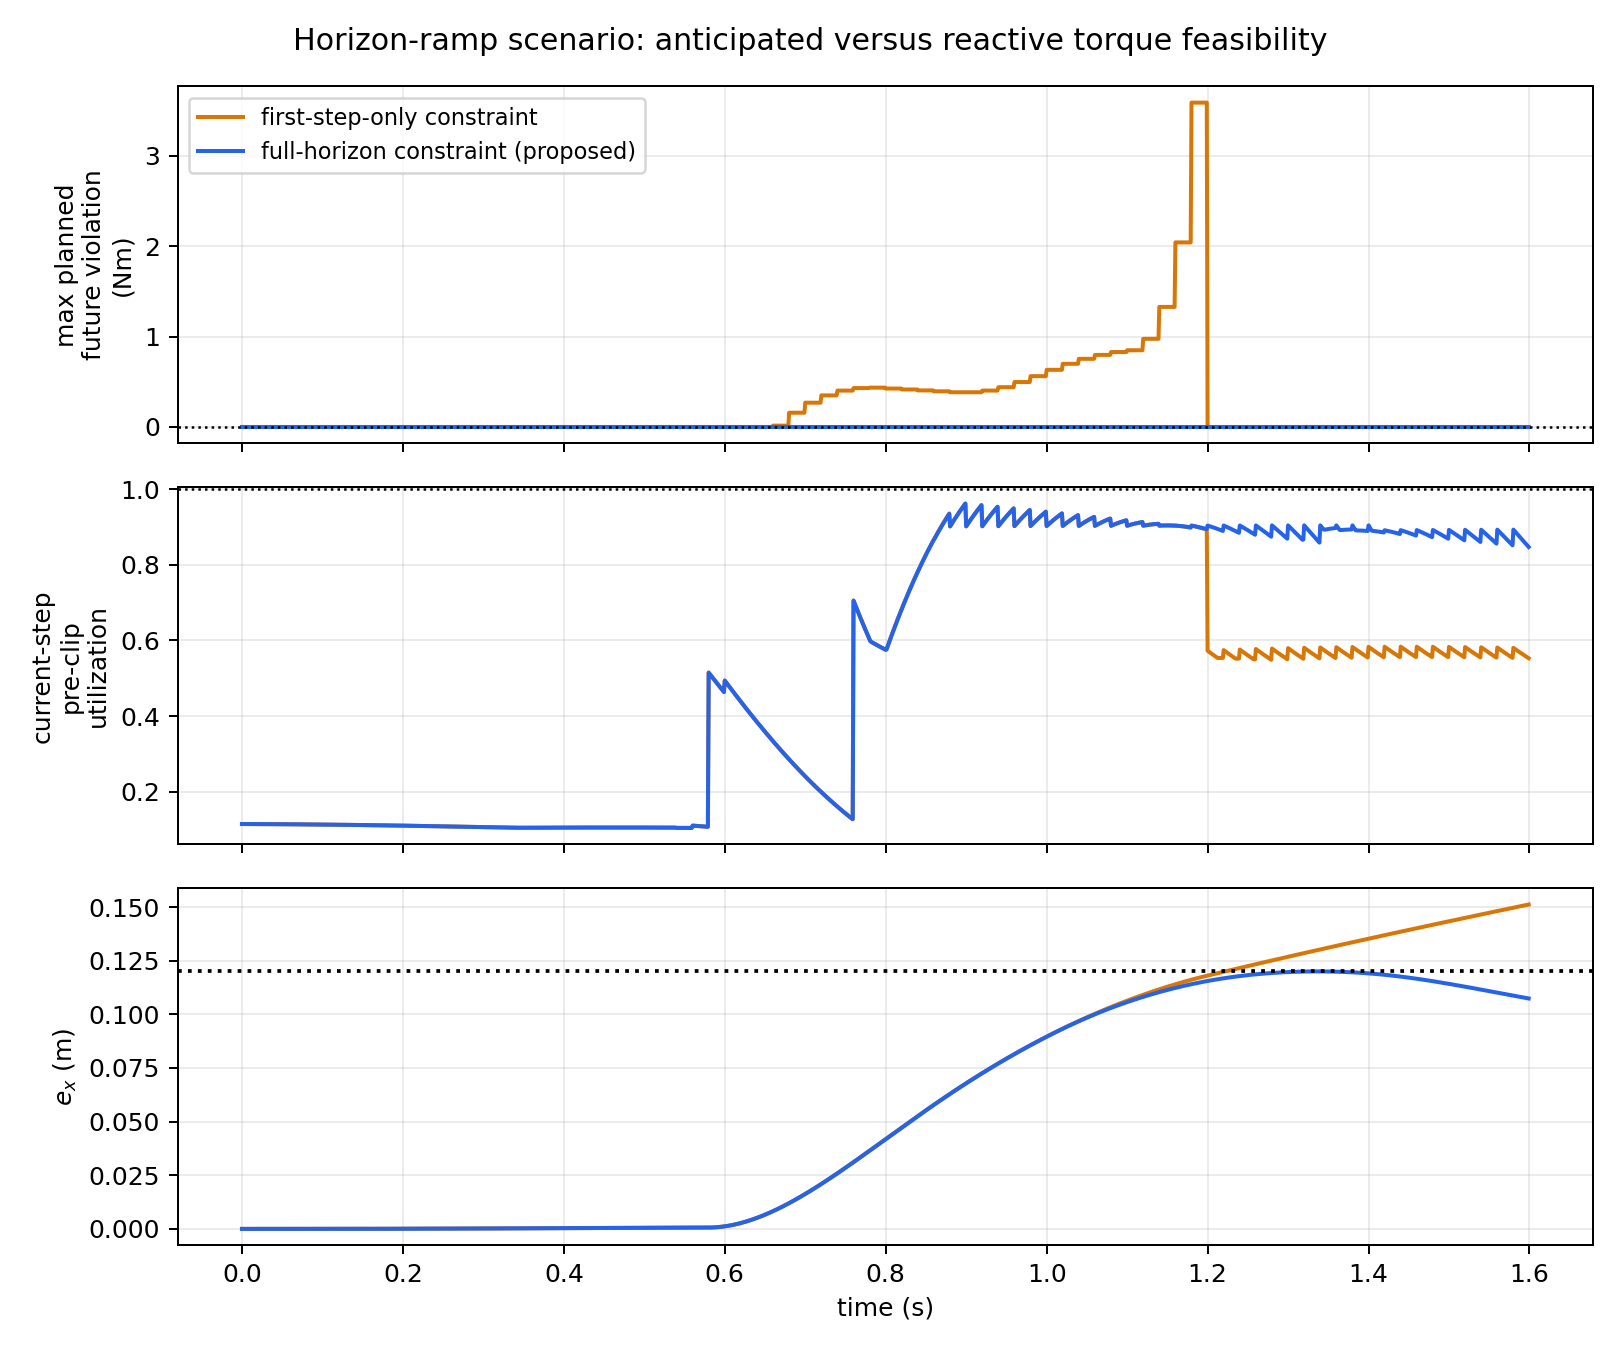
\includegraphics[width=\columnwidth]{horizon_ramp_results.png}
\caption{Horizon-ramp scenario: a first-step-only constraint sees a legal present and walks into an illegal future; the full-horizon constraint sees it coming.}
\label{fig:horizon}
\end{figure}

Fig.~\ref{fig:horizon} isolates why anticipation is a different constraint from reactive limiting, not a refinement of it:
\begin{itemize}
\item The manager's horizon rows query the scenario's scheduled actuator-budget drop directly, so Fig.~\ref{fig:horizon} demonstrates the horizon-versus-one-step mechanism under a known future constraint, not forecasting of an unknown one.
\item The first-step-only constraint's predicted future torque violation reaches 3.587~Nm; the full-horizon constraint stays at zero throughout.
\item The first-step-only variant's QP is feasible for only 75\% of updates, versus 100\% for the full-horizon variant.
\item The resulting 31.180~mm of workspace excess occurs entirely during the infeasible 25\%, mediated by the reactive fallback of Section~\ref{sec:predictivecorrection} (0.000~mm while the QP is feasible).
\end{itemize}

\begin{figure}[t]
\centering
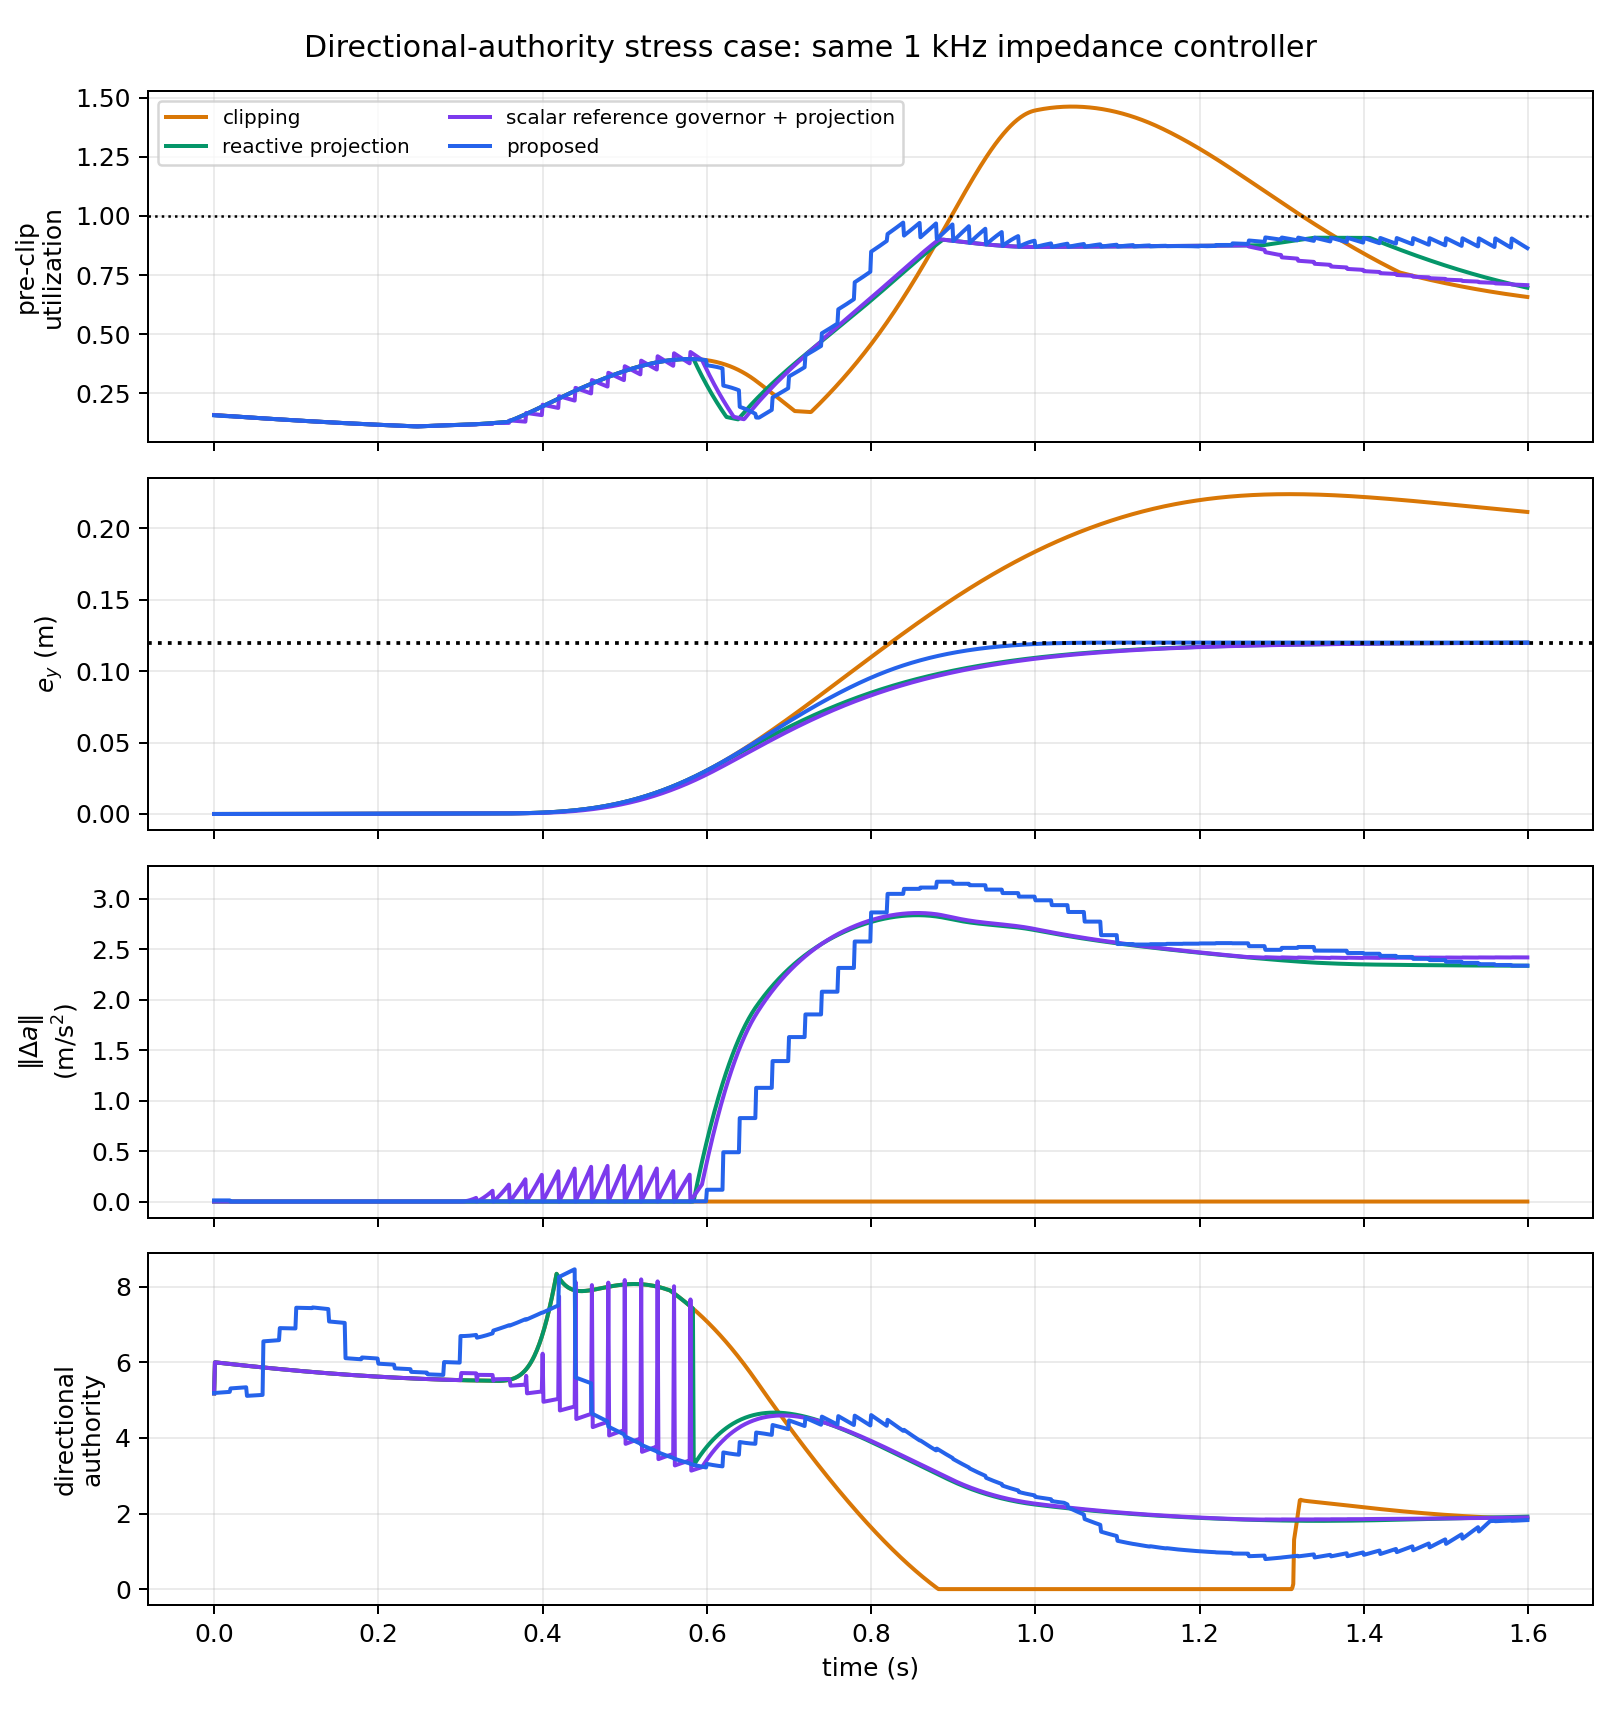
\includegraphics[width=0.8\columnwidth]{directional_authority_results.png}
\caption{Directional-authority stress case with a common impedance-controller interface.}
\label{fig:directional}
\end{figure}

Fig.~\ref{fig:directional} shows the directional-authority stress case. Direct clipping exceeds both the feasible request set and the workspace bound. The predictive methods intervene earlier, and the vector correction preserves the workspace constraint while leaving a visible intervention residual. Measured along the disturbance direction (metric defined in Appendix~\ref{app:params}), the proposed manager's authority reaches zero for about a fifth of the trajectory while the applied request keeps the workspace constraint satisfied throughout; the reactive projection and matched horizon reference governor retain positive authority in this direction across the whole run (minimum 1.82 and 1.87~m/s$^2$).

\begin{figure}[t]
\centering
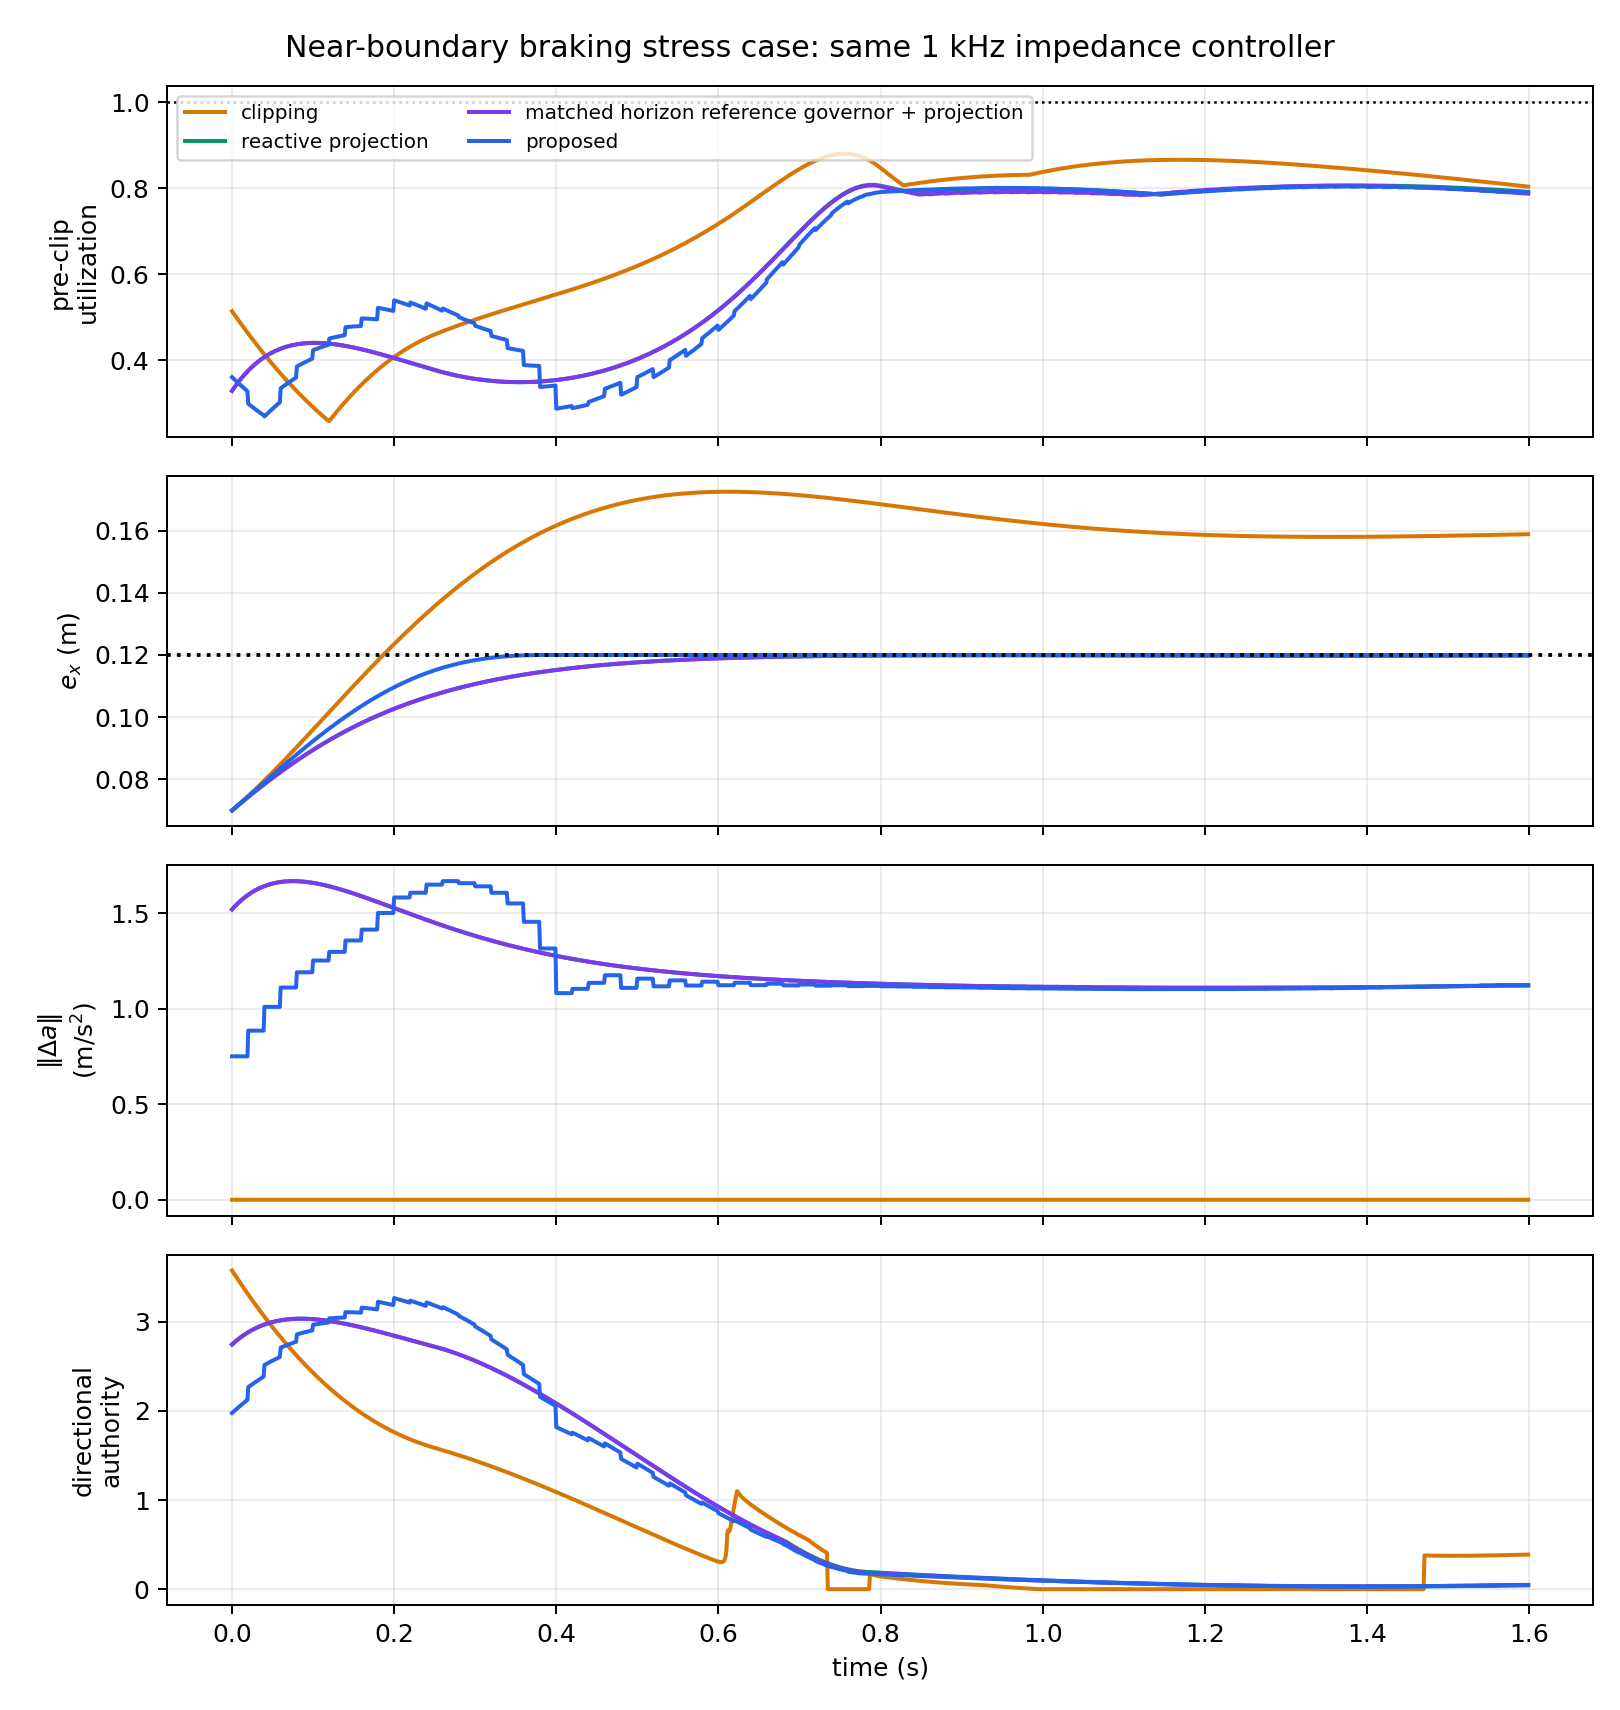
\includegraphics[width=0.8\columnwidth]{near_boundary_braking_results.png}
\caption{Near-boundary braking stress case; no viability kernel is inferred from this trajectory.}
\label{fig:braking}
\end{figure}

Fig.~\ref{fig:braking} shows near-boundary braking: an outward velocity close to the position boundary under a shrinking torque budget. Direct clipping overshoots the boundary and settles outside it. The reactive projection, matched horizon trajectory-reference governor plus projection, and proposed manager all arrest the position at the boundary. Because no viability kernel or terminal invariant set is computed, this supports finite-horizon constraint handling only.

Table~\ref{tab:scenarios} reports clipping, the matched horizon trajectory-reference governor, and the proposed behavior-coordinate manager across the remaining seven scenarios. The governor uses the same realization model, 20~ms update, 0.24~s horizon, actuator-limit schedule, tightening, and 1~kHz final projection. It searches one scalar reference multiplier, whereas the proposed manager optimizes an acceleration vector at each horizon step. This makes it an ERG-style same-model numerical comparator, not an exact reproduction of the Lyapunov/dynamic-safety-margin algorithm of \cite{r17}.

The two predictive architectures have the same qualitative outcome in the nominally successful cases: both remove pre-clip excess and hold workspace excess to numerical-scale values. Their intervention lead differs by at most 33~ms, comparable to two shared 20~ms manager updates; the horizon is $N\Delta t=0.24$~s. Correction RMSE (governor/proposed) is $1.124/1.060$, $1.389/1.401$, and $0.878/0.844~\mathrm{m/s^2}$ in slow saturation, directional collapse, and near-boundary braking, respectively; in the horizon-ramp isolation case it is $0.695/0.506~\mathrm{m/s^2}$. Thus the vector interface changes the requested behavior less in three of these four cases, while the scalar governor is marginally lower in directional collapse. This is evidence of a representation-dependent tradeoff, not general superiority over \cite{r17}, the generalized action governor \cite{r18}, or predictive safety filters \cite{r5,r16}.

\begin{table*}[t]
\caption{Same-Model Scenario Comparison. C/G/P Denotes Clipping/Matched Horizon Trajectory-Reference Governor/Proposed Behavior-Coordinate Manager.}
\label{tab:scenarios}
\centering
\footnotesize
\setlength{\tabcolsep}{4pt}
\begin{tabular}{@{}lccccc@{}}
\toprule
Scenario & \shortstack{Pre-clip\\C/G/P (Nm)} & \shortstack{Workspace\\C/G/P (mm)} & \shortstack{Lead\\G/P (s)} & \shortstack{P\\feasible} & \shortstack{P\\audit} \\
\midrule
No saturation & 0.000 / 0.000 / 0.000 & 0.000 / 0.000 / 0.000 & -- / -- & 100\% & Yes \\
Slow saturation & 0.000 / 0.000 / 0.000 & 78.970 / 0.000 / 0.001 & 0.399 / 0.414 & 100\% & Yes \\
Sudden disturbance & 7.151 / 10.236 / 11.879 & 0.000 / 0.000 / 0.000 & 0.086 / 0.084 & 92.5\% & No \\
Directional collapse & 0.708 / 0.000 / 0.000 & 103.868 / 0.000 / 0.003 & 0.307 / 0.340 & 100\% & Yes \\
Near-boundary braking & 0.000 / 0.000 / 0.000 & 52.537 / 0.000 / 0.011 & 0.574 / 0.568 & 100\% & Yes \\
Model mismatch & 12.453 / 1.190 / 2.018 & 190.904 / 160.711 / 197.006 & 0.542 / 0.633 & 45.0\% & No \\
Preview mismatch & 19.777 / 3.537 / 4.428 & 190.513 / 357.209 / 346.871 & 0.173 / 0.169 & 40.0\% & No \\
\bottomrule
\end{tabular}
\\[2pt]
\raggedright\footnotesize Table II. Same-model scenario comparison. C/G/P denotes clipping/matched horizon trajectory-reference governor/proposed behavior-coordinate manager. Lead is relative to each predictive method's own first nominal-limit event; Appendix~\ref{app:params} explains the shared-event diagnostic.
\end{table*}

\textbf{Negative cases.} QP feasibility is 100\% in the four successful stress cases but only 92.5\%, 45.0\%, and 40.0\% under sudden disturbance, model mismatch, and preview mismatch, with the reactive fallback of Section~\ref{sec:predictivecorrection} carrying most of the resulting excess. Under preview mismatch, the correction acts on a force forecast that misses a sign change inside the horizon and workspace excess rises from 190.513 to 346.871~mm --- substantially worse than doing nothing; model mismatch is similarly worse, 197.006 versus 190.904~mm, because the feasible geometry is assembled along a wrong rollout. Under sudden disturbance the implemented preview holds the measured force constant, so an unannounced impulse pushes pre-clip excess from 7.151 to 11.879~Nm even though the final projection keeps applied torque legal. The audit rejects all three cases, flagging exactly where Theorem~\ref{thm:transfer}'s premises are not met.

\subsection{Controller-interface substitution}

\begin{figure}[t]
\centering
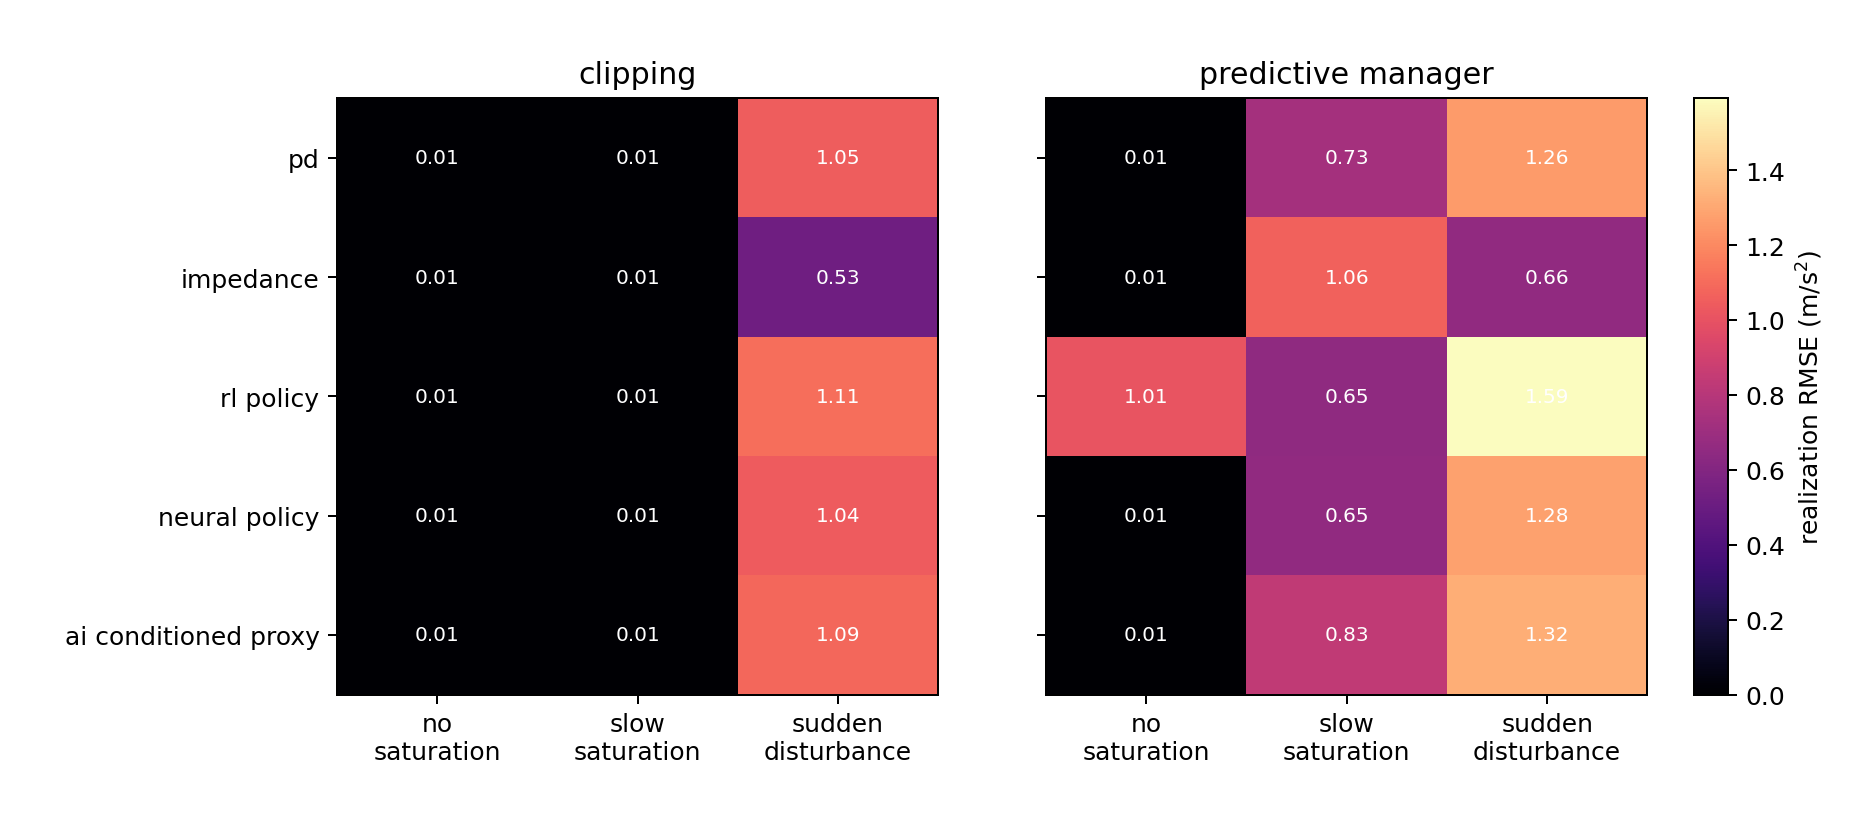
\includegraphics[width=\columnwidth]{controller_transfer.png}
\caption{Behavior-realization residuals for the five nominal-controller interfaces.}
\label{fig:controllers}
\end{figure}

As shown in Fig.~\ref{fig:controllers}, the manager formulation and weights are unchanged across interfaces. Under no saturation, correction RMSE is below 0.01~m/s$^2$ for four of five controllers; the small evolution-strategy policy is the exception at $\approx1.01~\mathrm{m/s^2}$ (bias source in Appendix~\ref{app:params}). The manager holds the state inside the workspace box but is compensating for a biased interface rather than remaining inactive. The case is kept as an interface stress test --- the architecture is not intended to repair behavior-policy quality, though its running constraints may incidentally reject a biased request.

Table~\ref{tab:controllers} separates the manager's deliberate correction ($a_{\mathrm{req}}-a^0$) from the tracking-defect RMSE ($a_{\mathrm{actual}}-a_{\mathrm{req}}$) most directly tied to certificate transfer. The tracking defect is 0.0111~m/s$^2$ for every interface --- a fixed, controller-independent unmodeled-error floor, since no clipping is active under slow saturation --- while correction RMSE varies with what each controller requests. All five cases pass the audit.

\begin{table}[t]
\caption{Controller Substitution Under Slow Saturation.}
\label{tab:controllers}
\centering
\footnotesize
\setlength{\tabcolsep}{3pt}
\setlength{\tabcolsep}{2pt}
\resizebox{\columnwidth}{!}{%
\begin{tabular}{@{}lcccc@{}}
\toprule
Interface & \shortstack{Correction\\RMSE (m/s$^2$)} & \shortstack{Tracking defect\\RMSE (m/s$^2$)} & \shortstack{Workspace\\excess (mm)} & Audit \\
\midrule
PD & 0.726 & 0.0111 & 0.001 & Pass \\
Impedance & 1.060 & 0.0111 & 0.001 & Pass \\
Trained policy & 0.652 & 0.0111 & 0.016 & Pass \\
Fitted neural policy & 0.649 & 0.0111 & 0.001 & Pass \\
Cond.\ motion primitive & 0.830 & 0.0111 & 0.006 & Pass \\
\bottomrule
\end{tabular}}
\end{table}

\subsection{Sampled interface audit across realization maps}
\label{sec:sampled}

\begin{table}[t]
\caption{Sampled Start/end Quantities Associated with the Three Conditions of Theorem~\ref{thm:transfer}.}
\label{tab:audit}
\centering
\footnotesize
\setlength{\tabcolsep}{3pt}
\begin{tabular}{@{}lccc@{}}
\toprule
Realization map & \shortstack{Max.\ T3 defect\\$\ell_\infty$ (m/s)} & \shortstack{Min.\ T1\\slack (Nm)} & \shortstack{Min.\ T2\\slack (Nm)} \\
\midrule
Planar 2R & 0.006815 & 0.007604 & 0.143756 \\
FR3-inspired surrogate & 0.006796 & 0.003888 & 0.646664 \\
Six-axis-arm surrogate & 0.006796 & 0.004871 & 0.707748 \\
\bottomrule
\end{tabular}
\end{table}

Each record is indexed by one feasible manager update, excluding ticks following an infeasible (fallback) solve since Theorem~\ref{thm:transfer} concerns the QP-optimized plan. (T1) and (T2) are evaluated at the beginning of the interval, using the manager's own first-horizon-step prediction $\hat\tau_0$ and the torque realized from that same request. Both use the same state, force, and request, though they are not numerically equal because their gap is exactly what (T1) bounds. The (T2) entry is that tick's first-step slack, not the horizon-wide minimum reported elsewhere. (T3) uses the physical state observed at the \emph{next} manager update. The table therefore reports a sampled start/end audit --- 316 records per robot from the no-saturation and slow-saturation cross-realization runs --- rather than asserting that its start-of-interval (T1) and (T2) values hold continuously while the fast controller and realization map evolve over the intervening 20~ms.

The pass/fail label in Tables~\ref{tab:scenarios} and~\ref{tab:controllers} comes from a separate, broader unpaired audit over every 1~kHz fast-loop sample. It uses a Euclidean (T3) bound, conservative relative to Table~\ref{tab:audit}'s $\ell_\infty$ value, checks the torque-error envelope, and directly requires realized pre-clip torque to remain inside the untightened actuator box. Thus the statement that pre-clip torque remains legal throughout each passing trajectory is supported by the fast-loop check, not inferred from Table~\ref{tab:audit}'s manager-update snapshots alone. Table~\ref{tab:audit} shows positive sampled slacks across all three realization maps: the (T3) defect remains below the 0.03~m/s certificate margin, while (T1) and (T2) retain room against $\bar\delta_\tau(a,F_h)$ (Appendix~\ref{app:params}). The true-plant coefficients are held out from the manager and are not generated by scaling the bound waveform itself. Nevertheless, both the coefficient box and held-out plants are synthetic; this is stronger than a self-envelope consistency check but remains weaker than an independently identified physical uncertainty set.

\subsection{Ablation summary and computation}
\label{sec:ablation}

\begin{figure}[t]
\centering
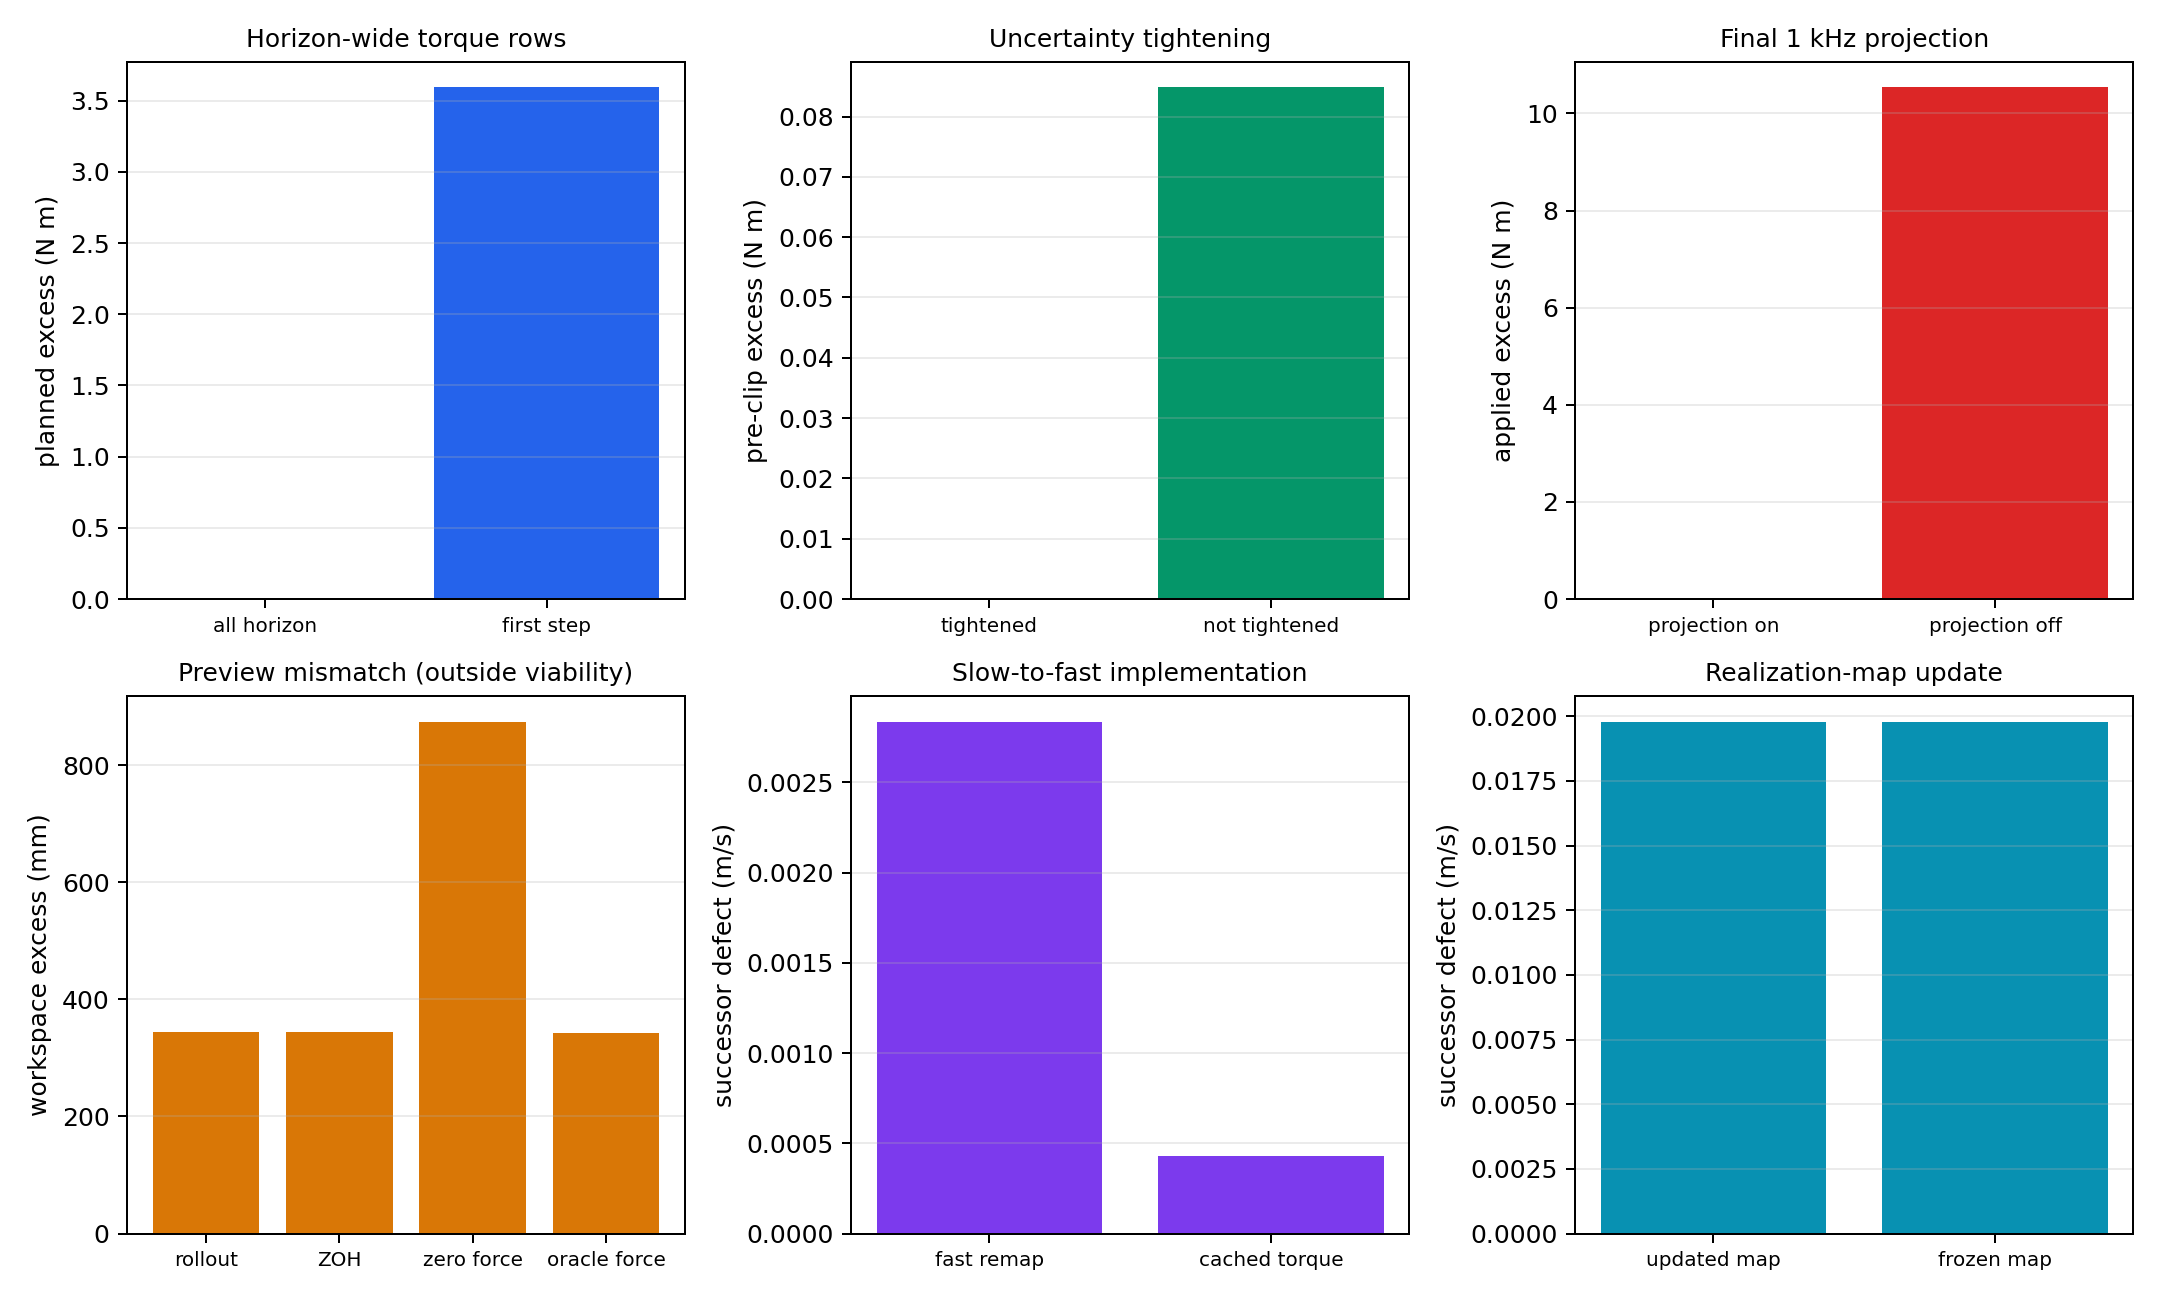
\includegraphics[width=\columnwidth]{ablation_summary.png}
\caption{Paired ablations of the predictive and fast-path implementation choices.}
\label{fig:ablation}
\end{figure}

Fig.~\ref{fig:ablation} isolates the four design choices central to the paper. Full-horizon enforcement keeps the horizon-ramp QP feasible and removes the 3.587~Nm planned violation left by first-step-only enforcement. Removing uncertainty tightening creates 0.0958~Nm of pre-clip excess; removing the final projection creates 10.456~Nm of applied excess under sudden disturbance. In the dedicated velocity-bound case, enforcing $\mathcal K_v$ limits peak speed to 0.5678~m/s, versus 0.5968~m/s without it. Appendix~\ref{app:params} gives the complete 17-run ablation ledger, secondary results, and wall-clock computation figures.

\section{Discussion}
\label{sec:discussion}

\emph{Scope of the contribution.} The double integrator, the QP, the ray-to-polytope authority calculation, and one-step certificate refinement are all established; none is claimed as new. What is offered is their arrangement into an interface with an explicit, online-checkable boundary between behavior preservation and physical realization, together with the conditions (T1)--(T3) that decide when that boundary holds. Theorem~\ref{thm:transfer} is a specialization of robust one-step refinement to this interface rather than a general certificate-transfer theorem, and the benchmark is a reduced-order synthetic study rather than a hardware evaluation.

The experiments support an interface claim, not the claim that a new safety controller works for every robot. The behavior-coordinate optimization and empirical audit threshold remain unchanged across the implemented controller interfaces and realization maps, while each map reconstructs its own feasible set and error bounds. This separation is the demonstrated contribution. It does not establish that an action governor or predictive safety filter could not use the same coordinates; Table I identifies that unresolved relationship explicitly.

Reference governors, action governors, and predictive safety filters could adopt the same behavior coordinates. What this implementation contributes is an explicit software and verification boundary: a behavior request and certified action set on one side; a robot-specific torque map, uncertainty margin, and successor audit on the other. In the present study the velocity certificate $(\mathcal S_v,\mathcal K_v,\epsilon_v)$ is deliberately minimal. The physical containment it requires --- that the real one-step mismatch stays inside $\epsilon_v$ --- is sampled along experiment trajectories rather than independently identified over the workspace. The torque audit separates the declared coefficient box from deterministic held-out true-plant coefficients, but both remain synthetic. The results therefore validate a held-out perturbation inside a prescribed uncertainty class and show audit rejection under constructed mismatch; they do not identify a workspace-wide physical uncertainty set.

The final high-rate projection is essential but should not be confused with behavior preservation: clipping protects the actuator but invalidates exact realization of the requested behavior. Theorem~\ref{thm:transfer} records sufficient conditions for clipping to remain inactive and for the velocity conclusion to hold for one transition. The mismatch experiments show these properties diverging. The matched horizon reference-governor comparison shows comparable constraint handling and a scenario-dependent correction tradeoff. Because neither a terminal invariant set nor an exact implementation of \cite{r17}, a generalized action governor, or a predictive safety filter is included, the results should not be read as recursive-safety or broad comparative-superiority evidence.

The three realization maps test software substitution and distinct actuator geometry inside one reduced-order model class. They do not demonstrate that an identified uncertainty contract or certificate transfers between physical robot dynamics. Corollary~\ref{cor:tworate} and the horizon-drift term of Section~\ref{sec:predictivecorrection} state the additional bounds such a claim would require; neither bound is identified by the present simulations.

\section{Conclusion}

This paper introduced a behavior-coordinate realization interface for predictive saturation management. The nominal controller exposes a task-acceleration request at its high servo rate; a slower manager forecasts robot-specific loss of realizability and modifies that request before clipping is required. Predictive supervision itself is established prior art. The contribution is the concrete separation between a reusable behavior-side request and action set and robot-specific objects that must be reconstructed and audited: the acceleration-to-torque map, actuator margin, uncertainty bounds, and operating region. A minimal velocity-certified action set is enforced inside the QP as an existence witness, while Theorem~\ref{thm:transfer} states the corresponding one-step realization contract.

Across 111 deterministic reduced-order runs, full-horizon enforcement eliminates a planned future violation that remains in the first-step-only variant, and the same interface accepts five nominal-controller forms. A sampled audit applies the same behavior-mismatch threshold while retaining distinct realization maps for three robot surrogates. Slow saturation, directional authority collapse, and near-boundary braking are handled within the tested region. A matched ERG-style trajectory-reference governor handles those constraints comparably; the vector behavior correction has lower correction RMSE in three of the four successful or horizon-isolation cases, but not in directional collapse. Abrupt disturbance and severe mismatch instead make the contract fail and frequently render the QP infeasible, leaving only the reactive fallback and final projection. These results establish that the interface operates, exposes a measurable representation tradeoff, and rejects assumptions as designed; they do not establish universal advantage over governor or safety-filter architectures.

The next decisive evaluations are exact reproductions of saturation-aware ERG, generalized action-governor, 
or predictive-safety-filter implementations and validation with independently identified error bounds on full 
rigid-body realizations. Extensions to position certificates and recursive feasibility are separate theoretical directions.

\appendices
\section{Benchmark Parameters}
\label{app:params}

This appendix lists the constants needed to reproduce the numbers in Section~\ref{sec:experiments}, including the complete ablation ledger; the full realization-map functions $H(x)$, $\tau_{\mathrm{base}}(x)$, the learned-policy weights, and the per-scenario timelines are in the simulation code released alongside this paper.

\textbf{Shared constants} (\texttt{BenchmarkConfig}, \texttt{simulation/saturation\_benchmark.py}): fast period $T_f=1$~ms, manager period $\Delta t=20$~ms, horizon $N=12$, episode duration 1.6~s, workspace box $\mathrm{pos}_{\max}=0.12$~m, speed box $v_{\max}=0.60$~m/s, acceleration bound $a_{\max}=12.0~\mathrm{m/s^2}$, acceleration rate bound $\dot a_{\max}=120.0~\mathrm{m/s^2/s}$, certificate/audit margin $\epsilon_v=\epsilon_{\mathrm{audit}}=0.03$~m/s, cost weights $W=1.0\cdot I$, $W_\Delta=0.025\cdot I$, OSQP tolerance $10^{-5}$. These give $\epsilon_v/\Delta t=1.5~\mathrm{m/s^2}$, well under $a_{\max}$ --- the concrete margin behind $\mathcal K_v$'s nonemptiness (Section~\ref{sec:certificate}).

\textbf{Realization maps} (torque limits in Nm, mass in kg): every listed torque-limit array is the positive magnitude $L$ of a symmetric box, $\tau_{\min}=-L$ and $\tau_{\max}=L$. Planar 2R --- 2 joints, $L=[9.0,7.5]$, mass 2.2; FR3-inspired surrogate --- 7 joints, $L=[16.0,13.0,12.0,15.0,6.0,6.0,4.5]$, mass 3.0; six-axis-arm surrogate --- 6 joints, $L=[12.0,10.0,9.0,8.5,5.5,4.5]$, mass 2.6. The interaction-error bound $\bar\delta_\tau$ uses base term 0.03~Nm per joint and the $H$-dependent term below, with $H_0=H(x)$ evaluated once at each map's zero-state configuration.

\textbf{Cross-realization audit detail.} Before the simulated true plants are instantiated, the manager's per-joint bound is fixed as
\begin{align*}
\bar\delta_\tau^{(j)}
=\ &s_{\mathrm{mm}}\Bigg(\underbrace{0.03}_{\text{Nm, base}} \\
&+0.008\sum_{k}\max\!\left(\left|H_0\right|_{jk},0.25\right)\left|a_k-\frac{F_{h,k}}{m}\right|\Bigg),
\end{align*}
where $s_{\mathrm{mm}}$ is the scenario's mismatch-scale multiplier (1.0 for the cross-realization cases reported here, up to 2.4 for model mismatch elsewhere in Section~\ref{sec:experiments}), ranging from 0.0300 to 0.0926~Nm over the audit; this is $\bar\delta_\tau(a,F_h)$, the action-dependent bound of Section~\ref{sec:realizable}, not the QP's own more conservative $\bar\delta_\tau^{\mathrm{QP}}$. The held-out true plants are then generated with seeds 31, 37, and 41 for planar 2R, FR3-inspired, and six-axis-arm maps. Their independent coefficients satisfy $|c_H|\le0.0065<0.008$ and base-error amplitudes in $[0.012,0.027]$~Nm${}<0.03$~Nm, with independently sampled phases and frequencies; these realized values are never passed to the manager. Table~\ref{tab:audit} reports the resulting (T1) and (T2) slacks directly. This is a deterministic held-out test within a prescribed synthetic coefficient box, not identification of that box from physical data.

\textbf{Baseline architectures.} Reactive 1~kHz projection: exact Euclidean projection onto the intersection of the current-step tightened torque halfspaces and a relative-degree-two box control-barrier-function halfspace set with decay rate $\lambda=8$ (\texttt{reactive\_state\_halfspaces}), i.e.\ position rows $\mp a\le\pm2\lambda v+\lambda^2(\mathrm{pos}_{\max}\mp p)$ and speed rows $\mp a\le\lambda(v_{\max}\mp v)$. Matched horizon trajectory-reference governor: at each manager tick, \texttt{governor\_scale} uses bisection to find the largest $\alpha\in[0,1]$. For each candidate it rolls the state through all $N=12$ steps, evaluates the nominal controller against $p+\alpha(p_r-p)$, and checks the same scheduled actuator limits, uncertainty-tightened torque halfspaces, workspace bound, measured-force hold, model, 20~ms update, and 0.24~s horizon as the proposed manager. One bound is deliberately \emph{not} matched: the governor is checked against the untightened speed limit $v_{\max}=0.60$~m/s, whereas the proposed manager additionally enforces the velocity certificate and is therefore held to $v_{\max}-\epsilon_v=0.57$~m/s, a 5\% tighter bound. The comparison is thus conservative toward the proposed method: its lower correction RMSE in Table~\ref{tab:scenarios} is obtained under a strictly smaller admissible set than the comparator enjoys. The first governed reference is held until the next manager tick and its requested acceleration is passed through the same reactive projection. This is an ERG-style same-model comparator motivated by \cite{r17}, but it directly searches finite-horizon constraint feasibility rather than reproducing \cite{r17}'s Lyapunov/dynamic-safety-margin law.

\textbf{Directional-authority metric.} $\alpha^+$ (Section~\ref{sec:reports}) is a function of a chosen direction $y$. Fig.~\ref{fig:directional} reports it along the fixed, exogenous disturbance direction rather than the manager's own correction direction, which is endogenous --- it can change discontinuously as the manager's own output changes --- and so is not directly comparable across methods or time; both use the same halfspace-ray construction.

\textbf{Governor-search validation.} The matched governor uses bisection over $\alpha$, which assumes feasibility is monotone in $\alpha$. A dense 201-point grid check across all 160 manager ticks at which the governor is invoked in this benchmark found no non-monotone case. A regression test additionally confirms that its horizon attenuates the reference before a scheduled limit drop that a one-step version cannot yet see.

\textbf{Controller interfaces.} PD and impedance are closed-form analytic laws. The trained policy is a small $\tanh$-squashed single-hidden-layer network fit by a deterministic evolution strategy. The fitted neural policy is an 18-unit $\tanh$ hidden layer with a linear output head, least-squares fit to impedance-law demonstrations (\texttt{saturation\_benchmark.py}, \texttt{RLPolicyController}/neural-controller fit). The conditioned motion primitive is a PD servo tracking a primitive-conditioned reference.

\textbf{Trained-policy bias (Section~\ref{sec:experiments}).} The evolution-strategy policy's limited training set does not cover the test trajectory symmetrically, and it retains a positive-$y$ command bias; this is an observed generalization error, not a specific failure of the evolution-strategy algorithm.

\textbf{Computation.} In the saved run, both the manager's and the fast path's worst observed wall-clock maxima remained below their nominal periods (20~ms and 1~ms respectively), with median solve times well under either budget. These are wall-clock measurements of computational cost on a development machine, not a real-time guarantee; because they are nondeterministic run-to-run, the released \texttt{results/all\_experiment\_metrics.json} is the source of record rather than any specific figure quoted here. The simulator itself advances the physical state by exactly 1~ms every step and does not model a scheduler that drops or delays steps on a missed deadline. A hard real-time implementation with an explicit scheduling policy is future work.

\textbf{Case accounting.} The 111 cases comprise 40 scenario cases, 30 controller-interface cases, 24 cross-realization cases, and 17 ablations grouped into eight families. The 40 scenario cases are eight scenarios evaluated with five channels: four architectures --- direct clipping, a reactive 1~kHz projection, the matched horizon trajectory-reference governor followed by the same reactive projection, and the proposed horizon-wide behavior-coordinate correction with final projection --- plus one unconstrained nominal-reference channel without torque projection. The stress scenarios are no saturation, slow saturation, sudden disturbance, directional authority collapse, near-boundary braking, model mismatch, preview mismatch, and a horizon-ramp scenario reported directly as Fig.~\ref{fig:horizon} and used for the constraint-width ablation of Section~\ref{sec:ablation}. A ninth scenario, starting inside $\mathcal S_v$ near its tightened boundary, is used only for the velocity-certificate ablation and enters neither the scenario nor the cross-realization matrices.

\textbf{Complete ablation ledger.} All ablations use the FR3-inspired surrogate and impedance controller.

\begin{table}[t]
\caption{Complete Ablation Ledger}
\label{tab:ablations}
\centering
\footnotesize
\setlength{\tabcolsep}{3pt}
\begin{tabular}{@{}rp{1.5cm}p{1.7cm}p{2.9cm}@{}}
\toprule
\# & Scenario & Variant & Changed element \\
\midrule
1 & Horizon ramp & Full & Complete proposed manager \\
2 & Horizon ramp & First-step torque & Torque constraints only at the first horizon step \\
3 & Slow saturation & Cached full torque & Hold the complete torque command between manager updates \\
4 & Sudden disturbance & Full & Complete proposed manager \\
5 & Sudden disturbance & No final projection & Disable the 1~kHz torque projection \\
6 & Model mismatch & Full & Complete proposed manager \\
7 & Directional collapse & Full & Complete proposed manager \\
8 & Directional collapse & No tightening & Set $\bar\delta_\tau=0$ in the predictive constraints \\
9 & Model mismatch & Frozen realization map & Freeze $H$ and $\tau_{\mathrm{base}}$ at the current manager state \\
10 & Model mismatch & Updated realization map & Evaluate the maps along the nominal predicted states \\
11 & Preview mismatch & Full & Measured-force hold preview \\
12 & Preview mismatch & Acceleration ZOH & Hold the current nominal acceleration over the horizon \\
13 & Preview mismatch & Zero-force preview & Set the forecast force to zero \\
14 & Preview mismatch & Oracle-force preview & Supply the scenario's future force \\
15 & Slow saturation & No smoothing & Set $W_\Delta=0$ \\
16 & Certificate-margin case & Constrained & Enforce $\mathcal K_v$ \\
17 & Certificate-margin case & Unconstrained & Remove $\mathcal K_v$ \\
\bottomrule
\end{tabular}
\end{table}

\textbf{Secondary ablation results.} Removing request smoothing leaves correction RMSE under slow saturation essentially unchanged (1.0603~m/s$^2$ without it versus 1.0604~m/s$^2$ with it). Zero-force preview increases workspace excess from 346.871 to 875.475~mm, but no preview option restores viability in the severe mismatch case. Recomputing the fast map does not outperform cached torque in this reduced-order benchmark, and updating it is numerically indistinguishable from freezing it. These are reported as non-results rather than evidence for those mechanisms.

\textbf{Reproducibility.} All code, tests, saved metrics, and figure-generation scripts are released alongside this paper. The complete configuration --- including the ablation-family definitions and scenario force/goal timelines --- is fixed in \texttt{simulation/saturation\_benchmark.py} and \texttt{simulation/run\_all\_experiments.py}. The evolution-strategy policy uses RNG seed 4, and the fitted neural policy uses seed 7. From the \texttt{pHRI/saturation} directory, the complete deterministic suite is regenerated with:
\begin{quote}
\scriptsize\ttfamily
python3 -m pip install -r requirements.txt\\
MPLCONFIGDIR=/tmp/mpl-saturation \textbackslash\\
\ \ XDG\_CACHE\_HOME=/tmp/cache-saturation \textbackslash\\
\ \ PYTHONPATH=simulation \textbackslash\\
\ \ python3 simulation/run\_all\_experiments.py
\end{quote}
The command writes \texttt{results/\allowbreak all\_experiment\_\allowbreak metrics.json}
and the figures used in Section~\ref{sec:experiments}.

\balance

\section{An A Priori Bound for Condition (T3)}
\label{app:t3bound}

Section~\ref{sec:certificate} verifies (T3) by measurement. This appendix
discharges the decomposition sketched there into an \emph{a priori} sufficient
condition: if the five constants below are known for a given robot and
operating region, (T3) holds without being checked online. The benchmark of
Section~\ref{sec:experiments} does not evaluate these constants --- it measures
the aggregate defect instead --- so what follows is a route to replacing that
measurement, not a description of it.

\subsection{Assumptions}

Throughout, $\mathcal O$ denotes the verified operating region, all norms are
$\ell_\infty$ on task quantities and induced norms on matrices, and $\Delta t$
is the manager period with $T_f$ the fast period ($\Delta t=n_fT_f$).

\begin{enumerate}
\item[(A1)] \textbf{Regularity.} $J(q)$ has full row rank on $\mathcal O$ with
$\lambda_{\min}(JM^{-1}J^\top)\ge\underline\lambda>0$ and
$\lambda_{\max}(JM^{-1}J^\top)\le\bar\lambda$; also
$\sigma_{\max}(J)\le\bar\sigma_J$ and $\lambda_{\min}(M)\ge\underline\mu>0$.
This is the standing assumption of Section~\ref{sec:realizable}, quantified.
\item[(A2)] \textbf{Bounded motion.} $\|\dot x\|\le V_x$ on $\mathcal O$.
\item[(A3)] \textbf{Lipschitz realization.} The map from state to realized task
acceleration under a held torque is Lipschitz on $\mathcal O$ with constant
$L_a$; that is, holding $\tau$ fixed, $\|\ddot p(x)-\ddot p(x')\|\le L_a\|x-x'\|$.
\item[(A4)] \textbf{Secondary-torque consistency defect.}
$\|JM^{-1}N_\tau\|\le\kappa_{\mathrm{sec}}$ and
$\|\tau_{\mathrm{sec}}\|\le T_{\mathrm{sec}}$ on $\mathcal O$. Exact dynamic
consistency is $\kappa_{\mathrm{sec}}=0$.
\item[(A5)] \textbf{Bounded model errors.} The force-model error satisfies
$\|\delta_F\|\le\bar\delta_F$ and the torque-realization error
$\|\delta_\tau\|\le\bar\delta_\tau$, the latter being the same bound already
used for tightening in (T1)--(T2).
\end{enumerate}

\subsection{The bound}

\begin{proposition}[A priori (T3) satisfaction]
\label{prop:t3}
Let the manager hold its correction over $[t_k,t_{k+1}]$ and let $\bar a_k$ be
the interval-averaged request of Corollary~\ref{cor:tworate}. Under
\textnormal{(A1)--(A5)}, if
\begin{equation}
\Delta t\left(\eta_{\mathrm{disc}}+\eta_{\mathrm{hold}}
+\eta_{\mathrm{sec}}+L_F\bar\delta_F+L_\tau\bar\delta_\tau\right)
\ \le\ \epsilon_v ,
\label{eq:t3bound}
\end{equation}
with the five terms given by
\begin{align}
\eta_{\mathrm{disc}}&=L_aV_xT_f, &
\eta_{\mathrm{hold}}&=\sup_{t}\|a_f(t)-\bar a_k\|, \nonumber\\
\eta_{\mathrm{sec}}&=\kappa_{\mathrm{sec}}T_{\mathrm{sec}}, &
L_F&=\bar\lambda, \nonumber\\
L_\tau&=\bar\sigma_J/\underline\mu, & &
\label{eq:t3terms}
\end{align}
then \textnormal{(T3)} holds for that interval, and the conclusion of
Theorem~\ref{thm:transfer} follows without measuring the successor defect.
\end{proposition}

\begin{IEEEproof}
Write the realized task acceleration as $\ddot p(t)=\bar a_k+e(t)$. Since the
abstract successor is $F_v(\Pi(x_k),\bar a_k)=v_k+\Delta t\,\bar a_k$ and the
physical successor is $v_k+\int_{t_k}^{t_{k+1}}\ddot p(t)\,dt$, the (T3) defect
is exactly $\bigl\|\int_{t_k}^{t_{k+1}}e(t)\,dt\bigr\|\le\Delta t\sup_t\|e(t)\|$.
It remains to bound $\|e(t)\|$ by the bracketed sum.

By (A1) the realization law \eqref{eq:iv0a} gives $\ddot p=a$ exactly when the
model is exact, the torque is unclipped --- guaranteed here by (T1)--(T2) --- and
the map is evaluated at the current state. Each bracketed term is one departure
from that identity, and the departures are additive in acceleration:

\emph{Discretization.} Within a fast period the realization map is held at its
value at the sample instant while the state moves by at most $V_xT_f$ by (A2);
(A3) converts this to an acceleration error $L_aV_xT_f$.

\emph{Hold.} The manager predicts with the single value $\bar a_k$ while the
fast loop applies $a_f(t)$; the instantaneous discrepancy is
$\|a_f(t)-\bar a_k\|$ by definition. (Its integral vanishes by the definition of
$\bar a_k$, so this term may be replaced by zero when the QP is posed on the
interval average; it is retained for implementations that predict with
$a_f(t_k)$.)

\emph{Secondary torque.} The secondary term contributes $JM^{-1}N_\tau\tau_{\mathrm{sec}}$
to task acceleration, which is zero under exact dynamic consistency and at most
$\kappa_{\mathrm{sec}}T_{\mathrm{sec}}$ under (A4).

\emph{Force model.} An uncompensated force error $\delta_F$ enters task
acceleration through $\Lambda^{-1}=JM^{-1}J^\top$, whose norm is at most
$\bar\lambda$ by (A1), giving $\bar\lambda\bar\delta_F$.

\emph{Torque.} A torque error $\delta_\tau$ enters through $JM^{-1}$, and
$\|JM^{-1}\|\le\sigma_{\max}(J)/\lambda_{\min}(M)\le\bar\sigma_J/\underline\mu$
by (A1), giving $(\bar\sigma_J/\underline\mu)\bar\delta_\tau$.

Summing and multiplying by $\Delta t$ yields \eqref{eq:t3bound}.
\end{IEEEproof}

\subsection{Reading the bound}

Three properties are worth noting.

First, \eqref{eq:t3bound} is \emph{sufficient, not necessary}: it bounds each
source by its worst case over $\mathcal O$ and adds them, so it is conservative
by construction. A measured defect well inside the budget --- as in
Section~\ref{sec:sampled} --- is consistent with \eqref{eq:t3bound} being tight
or violated, and the two are not interchangeable evidence.

Second, the bound is \emph{actionable in design}. Every term is a quantity a
designer controls: $\eta_{\mathrm{disc}}$ falls linearly with the fast period,
$\eta_{\mathrm{hold}}$ vanishes if the QP is posed on the interval average,
$\eta_{\mathrm{sec}}$ vanishes under exact dynamic consistency, and the last two
scale linearly with the declared force- and torque-error boxes. The manager
period enters as an overall factor, which is the formal counterpart of the
empirical observation that the slower rate is adequate only over a restricted
operating region.

Third, it \emph{closes the loop with (T1)}. The same $\bar\delta_\tau$ that
tightens the actuator box in (T2) appears in the last term, so a single declared
torque-error budget governs both the actuator margin and the certificate margin;
they cannot be tuned independently.

Establishing the constants $L_a$, $V_x$, $\kappa_{\mathrm{sec}}$, $\bar\lambda$,
$\bar\sigma_J$ and $\underline\mu$ for a full rigid-body robot over a stated
operating region is an identification task this paper does not perform, and it is
the substantive obstacle between the audited interface reported here and a
deployment-time guarantee.


\begin{thebibliography}{21}

\bibitem{r1} N.~Hogan, ``Impedance Control: An Approach to Manipulation---Part I: Theory,'' \emph{J. Dyn. Syst. Meas. Control}, vol.~107, no.~1, pp.~1--7, 1985.

\bibitem{r2} O.~Khatib, ``A Unified Approach for Motion and Force Control of Robot Manipulators: The Operational Space Formulation,'' \emph{IEEE J. Robot. Autom.}, vol.~3, no.~1, pp.~43--53, 1987.

\bibitem{r3} E.~Garone, S.~Di Cairano, and I.~Kolmanovsky, ``Reference and Command Governors for Systems with Constraints: A Survey on Theory and Applications,'' \emph{Automatica}, vol.~75, pp.~306--328, 2017.

\bibitem{r4} A.~D. Ames, S.~Coogan, M.~Egerstedt, G.~Notomista, K.~Sreenath, and P.~Tabuada, ``Control Barrier Functions: Theory and Applications,'' in \emph{Proc. Eur. Control Conf. (ECC)}, 2019, pp.~3420--3431.

\bibitem{r5} K.~P. Wabersich and M.~N. Zeilinger, ``Linear Model Predictive Safety Certification for Learning-Based Control,'' in \emph{Proc. IEEE Conf. Decis. Control (CDC)}, 2018.

\bibitem{r6} Y.-Y. Cao, Z.~Lin, and D.~G. Ward, ``An Anti-Windup Approach to Enlarging Domain of Attraction for Linear Systems Subject to Actuator Saturation,'' \emph{IEEE Trans. Autom. Control}, vol.~47, no.~1, pp.~140--145, 2002.

\bibitem{r7} Y.-Y. Cao, Z.~Lin, and D.~G. Ward, ``Anti-Windup Design of Output Tracking Systems Subject to Actuator Saturation and Constant Disturbances,'' \emph{Automatica}, vol.~40, no.~7, pp.~1221--1228, 2004.

\bibitem{r8} A.~Girard and G.~J. Pappas, ``Approximation Metrics for Discrete and Continuous Systems,'' \emph{IEEE Trans. Autom. Control}, vol.~52, no.~5, pp.~782--798, 2007.

\bibitem{r9} A.~Girard and G.~J. Pappas, ``Hierarchical Control System Design Using Approximate Simulation,'' \emph{Automatica}, vol.~45, no.~2, pp.~566--571, 2009.

\bibitem{r10} P.~Nuzzo, J.~B. Finn, A.~Iannopollo, and A.~Sangiovanni-Vincentelli, ``Contract-Based Design of Control Protocols for Safety-Critical Cyber-Physical Systems,'' in \emph{Proc. Des. Autom. Test Eur. (DATE)}, 2014.

\bibitem{r11} M.~Sharifi, S.~Behzadipour, and G.~Vossoughi, ``Nonlinear Model Reference Adaptive Impedance Control for Human--Robot Interactions,'' \emph{Control Eng. Pract.}, vol.~32, pp.~9--27, 2014.

\bibitem{r12} L.~Roveda, A.~Testa, A.~A. Shahid, F.~Braghin, and D.~Piga, ``Q-Learning-Based Model Predictive Variable Impedance Control for Physical Human--Robot Collaboration,'' \emph{Artif. Intell.}, vol.~312, art.~103771, 2022.

\bibitem{r13} K.~Haninger, C.~Hegeler, and L.~Peternel, ``Model Predictive Impedance Control with Gaussian Processes for Human and Environment Interaction,'' \emph{Robot. Auton. Syst.}, vol.~165, art.~104431, 2023.

\bibitem{r14} A.~S. Anand, J.~T. Gravdahl, and F.~J. Abu-Dakka, ``Model-Based Variable Impedance Learning Control for Robotic Manipulation,'' \emph{Robot. Auton. Syst.}, vol.~170, art.~104531, 2023.

\bibitem{r15} J.~Xue, W.~Liang, Y.~Wu, and T.~H. Lee, ``Model Predictive Variable Impedance Control Towards Safe Robotic Interaction in Unknown Disturbance-Rich Environments,'' \emph{Robot. Auton. Syst.}, vol.~189, art.~104961, 2025.

\bibitem{r16} K.~P. Wabersich and M.~N. Zeilinger, ``A Predictive Safety Filter for Learning-Based Control of Constrained Nonlinear Dynamical Systems,'' \emph{Automatica}, vol.~129, art.~109597, 2021.

\bibitem{r17} M.~Ambrosino, A.~Cotorruelo, and E.~Garone, ``A Saturation-Aware Trajectory-Based Explicit Reference Governor for a Robotic Arm,'' in \emph{Proc. IEEE/RSJ Int. Conf. Intell. Robots Syst. (IROS)}, 2022, pp.~13641--13646.

\bibitem{r18} P.~Fang, W.~Zhang, L.~Xiong, N.~Li, Y.~Huang, Y.~Li, I.~Kolmanovsky, A.~Girard, H.~E. Tseng, and D.~Filev, ``Safe Control and Learning Using Generalized Action Governor,'' arXiv:2211.12628, submitted 2022, revised 2026.

\bibitem{r19} N.~Bousias, C.~Stamouli, A.~Tsiamis, and G.~J. Pappas, ``On Transferring Safety Certificates Across Dynamical Systems,'' arXiv:2602.03987, 2026.

\bibitem{r20} A.~Skuric, V.~Padois, and D.~Daney, ``Pycapacity: A Real-Time Task-Space Capacity Calculation Package for Robotics and Biomechanics,'' \emph{J. Open Source Softw.}, vol.~8, no.~89, art.~5670, 2023.

\bibitem{r21} Y.~Gautam, G.~Briscoe-Martinez, A.~Mohan, N.~Nechyporenko, A.~Roncone, and M.~M. Nicotra, ``Compliant Explicit Reference Governor for Contact Friendly Robotic Manipulators,'' arXiv:2504.09188, submitted 2025, revised 2026.

\end{thebibliography}

\end{document}
